\documentclass[11pt,a4paper]{article}

% ---------- fontes ----------
\usepackage{fontspec}
\setmainfont{texgyreheros}[
  Extension = .otf,
  UprightFont = *-regular,
  BoldFont = *-bold,
  ItalicFont = *-italic,
  BoldItalicFont = *-bolditalic,
]
% Latin Modern Mono em vez de Berkeley Mono: a licenca da Berkeley Mono impede a incorporacao no PDF
\setmonofont{lmmono10-regular}[Extension=.otf, BoldFont=lmmonolt10-bold, ItalicFont=lmmono10-italic]
\usepackage[brazil]{babel}

% ---------- layout no formato da Etapa 1 ----------
\usepackage{geometry}
\geometry{a4paper, left=2.5cm, right=2.5cm, top=3.6cm, bottom=2.5cm, headheight=1.6cm, headsep=0.8cm}
\usepackage{setspace}
\setstretch{1.15}
\setlength{\parindent}{0pt}
\setlength{\parskip}{6pt}

\usepackage{amsmath}
\usepackage{booktabs}
\usepackage{array}
\usepackage{tabularx}
\usepackage{graphicx}
\graphicspath{{images/}}
\usepackage{float}
\usepackage{enumitem}
\usepackage{etoolbox}
\usepackage{xcolor}
\definecolor{mackred}{RGB}{204,32,39}
\usepackage{tikz}
\usetikzlibrary{positioning, arrows.meta}
\usepackage[hidelinks]{hyperref}
\usepackage{xurl}
\urlstyle{same}
\setlength{\emergencystretch}{3em}

\usepackage[labelsep=endash, font=small, justification=centering, singlelinecheck=false]{caption}
\captionsetup[table]{position=top}
\captionsetup[figure]{position=top}
\newcommand{\nota}[1]{\par\vspace{2pt}{\small Nota: #1}}

\AtBeginEnvironment{table}{\setstretch{1}}
\AtBeginEnvironment{figure}{\setstretch{1}}

% titulos simples, em negrito
\usepackage{titlesec}
\titleformat{\section}{\normalfont\large\bfseries}{\thesection}{0.5em}{}
\titleformat{\subsection}{\normalfont\bfseries}{\thesubsection}{0.5em}{}
\titleformat{\subsubsection}{\normalfont\bfseries}{\thesubsubsection}{0.5em}{}
\titlespacing*{\section}{0pt}{18pt}{8pt}
\titlespacing*{\subsection}{0pt}{14pt}{6pt}
\titlespacing*{\subsubsection}{0pt}{10pt}{4pt}

% cabecalho com o logo EaD/Mackenzie e numero de pagina no rodape
\usepackage{fancyhdr}
\pagestyle{fancy}
\fancyhf{}
\fancyhead[C]{
\includegraphics[height=1.3cm]{logo_ead_mackenzie.png}}
\fancyfoot[C]{\small\thepage}
\renewcommand{\headrulewidth}{0pt}
\fancypagestyle{plain}{\fancyhf{}\fancyhead[C]{
\includegraphics[height=1.3cm]{logo_ead_mackenzie.png}}\fancyfoot[C]{\small\thepage}\renewcommand{\headrulewidth}{0pt}}
\fancypagestyle{capa}{\fancyhf{}\fancyhead[C]{
\includegraphics[height=1.3cm]{logo_ead_mackenzie.png}}\renewcommand{\headrulewidth}{0pt}}

\addto\captionsbrazil{%
  \renewcommand{\contentsname}{Sumário}%
  \renewcommand{\listfigurename}{Lista de figuras}%
  \renewcommand{\listtablename}{Lista de tabelas}%
}
\newcommand{\col}[1]{\texttt{#1}}

\begin{document}

% =====================================================================
% CAPA (mesmo modelo da Etapa 1)
% =====================================================================
\thispagestyle{capa}
\begin{center}
{\Large\color{gray!80!black} Etapa II}
\end{center}
\vspace{4pt}
{\setstretch{1.4}
\begin{tabular}{@{}>{\raggedleft\arraybackslash\color{gray!80!black}}p{5.6cm}|p{9.6cm}@{}}
\hline
COMPONENTE CURRICULAR & Projeto Aplicado I \\
\hline
 & \textbf{Grupo 9} \\
 & Caio Felipe Correa (10764072) \\
GRUPO & Jennifer Lins Baia da Silva (10756227) \\
 & Nilton Cesar Marques dos Santos (10733175) \\
\end{tabular}\par}
\vspace{-4pt}
{\color{mackred}\rule{\textwidth}{2.5pt}}

\vspace{0.8cm}
Github: \url{https://github.com/nltncsr/clique-economia-prefeitura-curitiba-insights}

\vspace{2.5cm}
\begin{center}
{\fontsize{26}{34}\selectfont\bfseries Projeto: Análise da variabilidade de preço de itens essenciais em supermercados de uma capital brasileira\par}
\vspace{0.8cm}
{\large Proposta analítica e análise exploratória de dados}
\end{center}
\clearpage

\tableofcontents
\listoffigures
\listoftables
\clearpage

\section{Introdução}

O programa Clique Economia, gerido pela Prefeitura de Curitiba, faz uma pesquisa diária de preços nos supermercados da cidade e disponibiliza os resultados no portal de dados abertos municipal, para auxiliar a pesquisa de preços pelo cidadão (PREFEITURA..., [20--]). A versão do conjunto usada neste trabalho foi obtida no Kaggle (PAULOGLADSON, [20--]) e tem 4.396.534 registros, de 01/03/2019 a 11/09/2026.

O objetivo deste trabalho é elaborar uma análise exploratória dos preços de itens essenciais coletados pelo Clique Economia entre 2019 e 2026, para identificar como esses preços variam no tempo e entre redes. O tema se liga ao ODS 2 (Fome Zero e Agricultura Sustentável), pelo custo da cesta básica, e ao ODS 10 (Redução das Desigualdades), pelas diferenças de preço entre redes. O código da análise está no notebook \col{scripts/exploration.ipynb} do repositório do grupo.

\section{Proposta analítica}

\subsection{Apresentação da organização}

Os dados são coletados pela Secretaria Municipal de Segurança Alimentar e Nutricional e disponibilizados pela Prefeitura de Curitiba por meio do programa Clique Economia (PREFEITURA..., [20--]). A base é atualizada periodicamente com novas coletas e identifica cada registro pelo nome da rede de supermercados e por um código de filial.

A base cobre 100 nomes de rede distintos (depois reduzidos a 79, por correção de grafia), para 93 identificadores de empresa. Esses números, assim como as demais estatísticas detalhadas deste documento sobre as colunas originais, vêm da amostra de cerca de 10\% do conjunto completo usada na análise (seção 3.1): a maioria das empresas na amostra opera sob um único nome de rede (65,59\%), mas 30,11\% aparecem sob dois nomes e 4,30\% sob três, geralmente por filiais com grafias diferentes do mesmo identificador. Essa inconsistência de nomes molda boa parte das limitações descritas na seção 2.6.

\subsection{Problema do estudo}

A consulta diária do Clique Economia mostra onde um item está mais barato hoje. Com sete anos de coletas, é possível responder perguntas que essa consulta não responde:

\begin{enumerate}[label=\alph*), itemsep=0pt, topsep=2pt]
  \item como o preço dos itens de uma cesta básica padronizada evoluiu entre 2019 e 2026?
  \item há redes consistentemente mais baratas ou mais caras para essa cesta?
  \item quanto custa a cesta em cada rede e qual é a diferença entre a mais barata e a mais cara?
  \item quais itens mais contribuíram para a alta ou a queda do custo da cesta em um dado período?
  \item quais registros são erros de coleta e quais são preços legítimos fora do padrão?
\end{enumerate}

O problema segue os pilares do pensamento computacional. A decomposição separa as cinco perguntas acima, que são os eixos da proposta. O reconhecimento de padrões busca tendências nas séries e redes que se repetem nos extremos do ranking. A abstração descarta \col{preco\_atacado\_qtd}, que vale sempre zero, e \col{codigo\_categoria}, que não tem dicionário, e reduz os quatro preços a um único preço efetivo. O algoritmo é o \textit{pipeline} da seção 2.5. A comparação por bairro, prevista na Etapa 1, saiu do escopo porque a base não informa o endereço dos estabelecimentos.

\subsection{Metadados}

A Tabela~\ref{tab:metadados} traz os metadados do conjunto completo (arquivo original, antes de qualquer amostragem) e a Tabela~\ref{tab:dicionario} atualiza o dicionário de dados da Etapa 1 com o que a análise revelou, incluindo a classificação de cada variável e as colunas derivadas criadas durante o trabalho.

\begin{table}[H]
\caption{Metadados do conjunto de dados}
\label{tab:metadados}
\small
\begin{tabularx}{\textwidth}{@{}p{3.6cm}X@{}}
\toprule
\textbf{Aspecto} & \textbf{Descrição} \\
\midrule
Tipo de arquivo & CSV com separador ponto e vírgula (\col{final.csv}), compactado em ZIP (cerca de 56 MB) \\
Tamanho & 4.396.534 registros e 11 colunas originais \\
Origem & Portal de dados abertos da Prefeitura de Curitiba, via o programa Clique Economia (PREFEITURA..., [20--]); versão consolidada obtida no Kaggle (PAULOGLADSON, [20--]) \\
Proprietário & Prefeitura Municipal de Curitiba, por meio da SMSAN \\
Sensibilidade & Dado público, sem restrição de acesso \\
Validade temporal & Coletas de 01/03/2019 a 11/09/2026; a base é atualizada periodicamente com novas coletas \\
LGPD & Não há dado pessoal: os registros descrevem produtos, preços e estabelecimentos comerciais, sem identificar pessoas físicas \\
\bottomrule
\end{tabularx}
\end{table}

\begin{table}[H]
\caption{Dicionário de dados}
\label{tab:dicionario}
\small
\begin{tabularx}{\textwidth}{@{}p{4.1cm}X p{2.5cm}@{}}
\toprule
\textbf{Coluna} & \textbf{Descrição} & \textbf{Tipo} \\
\midrule
\col{data\_pesquisa} & Data da coleta do preço no estabelecimento & Data \\
\col{id\_empresa} & Identificador da filial. Não é único no conjunto: o mesmo número aparece em redes diferentes (seção 3.2) & Inteiro (ID), com nulos \\
\col{rede} & Nome da rede de supermercados, com variações de grafia & Texto (categórico) \\
\col{codigo\_categoria} & Código da categoria do produto (0 a 9), sem dicionário que explique cada código & Inteiro (ID), com nulos \\
\col{id\_produto} & Código do produto, em geral EAN-13; alguns itens usam códigos curtos & Inteiro (ID) \\
\col{descricao} & Nome, marca e tamanho do produto, em texto livre & Texto \\
\col{preco\_regular} & Preço padrão de venda & Decimal (R\$) \\
\col{preco\_atacado} & Preço para compra em quantidade & Decimal (R\$) \\
\col{preco\_atacado\_qtd} & Quantidade mínima para o preço de atacado; vale zero em todos os registros & Inteiro \\
\col{preco\_promocao} & Preço em oferta temporária & Decimal (R\$) \\
\col{preco\_fidelidade} & Preço exclusivo para clientes de programa de fidelidade & Decimal (R\$) \\
\midrule
\col{preco\_efetivo} & Coluna derivada: o preço que o consumidor comum paga, escolhido entre os quatro preços acima (seção 3.3) & Decimal (R\$) \\
\col{rede\_normalizada} & Coluna derivada: nome da rede após a correção de erros de grafia e duplicidade (seção 3.4) & Texto (categórico) \\
\col{item} & Coluna derivada: item da cesta básica a que o produto pertence, obtido a partir do início da descrição (seção 4.1) & Texto (categórico) \\
\col{qtd\_fracionamento} & Coluna derivada: tamanho da embalagem em gramas ou mililitros, extraído do final da descrição (seção 4.2) & Decimal \\
\col{preco\_unitario} & Coluna derivada: preço por quilograma ou litro, calculado a partir de \col{preco\_efetivo} e \col{qtd\_fracionamento} (seção 4.3) & Decimal (R\$) \\
\bottomrule
\end{tabularx}
\end{table}

\subsection{Proposta do que será desenvolvido}

Os eixos da Etapa 1 continuam, ampliados para cobrir os 13 itens da cesta básica usados pela metodologia do DIEESE em vez dos quatro itens anteriores: (a) séries mensais do preço por unidade de medida de cada item; (b) ranking de custo da cesta por rede; (c) custo mensal da cesta completa; (d) decomposição de quanto cada item contribuiu para a variação do custo; e (e) regras para separar erros de coleta de preços altos legítimos. Esta etapa entrega a limpeza dos dados, o preço efetivo, as regras de anomalia, as séries de preço por unidade de medida, o custo da cesta e a comparação da cesta entre redes. A narrativa de \textit{data storytelling} fica para a Etapa 3.

\subsection{\textit{Pipeline} de dados}

O arquivo completo é lido em blocos de 500 mil linhas, o que permite calcular as estatísticas de todos os registros sem carregá-lo inteiro na memória. As análises detalhadas das colunas originais usam uma amostra aleatória de cerca de 10\%, com semente fixa para que o resultado se repita; a análise da cesta básica, por usar poucos produtos, é recalculada sobre o conjunto completo (Figura~\ref{fig:pipeline}).

\begin{figure}[H]
\caption{\textit{Pipeline} de dados da análise}
\label{fig:pipeline}
\centering
\begin{tikzpicture}[
  node distance = 0.45cm and 0.6cm,
  etapa/.style = {draw, rounded corners=2pt, align=center, font=\footnotesize, minimum width=4.8cm, minimum height=0.9cm, fill=gray!8},
  futuro/.style = {etapa, dashed, fill=white},
  seta/.style = {-{Stealth[length=2mm]}, thick},
]
\node[etapa] (a) {1. Leitura do ZIP em blocos\\de 500 mil linhas};
\node[etapa, below=of a] (b) {2. Perfil do conjunto completo\\(nulos, mín./máx., média, desvio)};
\node[etapa, below=of b] (c) {3. Amostragem aleatória\\(cerca de 10\%, semente 42)};
\node[etapa, below=of c] (d) {4. Padronização de tipos\\(datas e identificadores)};
\node[etapa, below=of d] (e) {5. Exploração de consistência\\(produto, categoria, rede, preços)};
\node[etapa, right=1.3cm of a] (f) {6. Preço efetivo\\(prioridade entre os quatro preços)};
\node[etapa, below=of f] (g) {7. Seleção dos 13 itens da cesta\\e corte a partir de abril/2023};
\node[etapa, below=of g] (h) {8. Outliers pelo IQR\\(k=1,5, análise e remoção)};
\node[etapa, below=of h] (i) {9. Preço por unidade de medida\\(kg, litro ou dúzia)};
\node[etapa, below=of i] (j) {10. Recálculo sobre o dataset\\completo (etapas 6 a 9)};
\node[etapa, below=of j] (k) {11. Custo da cesta: mensal,\\por rede e por contribuição};
\node[futuro, below=of k] (l) {Etapa 3: \textit{storytelling}};
\draw[seta] (a) -- (b); \draw[seta] (b) -- (c); \draw[seta] (c) -- (d); \draw[seta] (d) -- (e);
\draw[seta] (e.east) -- ++(0.6,0) |- (f.west);
\draw[seta] (f) -- (g); \draw[seta] (g) -- (h); \draw[seta] (h) -- (i); \draw[seta] (i) -- (j);
\draw[seta] (j) -- (k);
\draw[seta, dashed] (k) -- (l);
\end{tikzpicture}
\end{figure}

\subsection{Limitações}

Além do que a Etapa 1 já apontava (só Curitiba e sem endereço dos estabelecimentos), a análise encontrou:

\begin{enumerate}[label=\alph*), itemsep=0pt, topsep=2pt]
  \item nomes de rede com variações de grafia e codificação (``Assai'' e ``Assaa''), sem identificador de rede para corrigi-los diretamente;
  \item códigos de categoria sem descrição;
  \item \col{preco\_atacado\_qtd} igual a zero em todos os registros;
  \item poucos registros em 2019 e 2020 (menos de 2\% do total);
  \item até março de 2023, a pesquisa registrava produtos genéricos, sem marca nem tamanho de embalagem, o que limita a comparação de preço por unidade de medida a partir de abril de 2023;
  \item a comparação entre redes, nos últimos 12 meses, cobre apenas as redes com pelo menos 20 registros de cada um dos 13 itens da cesta, cerca de 43\% das redes ativas no período (seção 5.4);
  \item apesar de \col{id\_empresa} identificar a filial dentro de cada rede, a base não traz bairro, região ou endereço da unidade. Algumas redes têm nome de bairro no próprio nome (por exemplo, uma filial identificada pelo bairro em que está instalada), mas essa informação aparece em uma fração pequena e inconsistente das redes, insuficiente para sustentar uma análise de variação de custo por região; a comparação neste trabalho fica restrita à evolução histórica e à comparação entre redes;
  \item depois da seleção do subtipo exigido pela metodologia do DIEESE (seção 4.1), alguns itens ficam com poucos produtos distintos no conjunto completo, como batata e pão (1 produto cada) e banana e tomate (2 produtos cada). Essa cobertura baixa é inerente ao próprio item, não à metodologia: batata, tomate e banana são vegetais, legumes e frutas, vendidos sem marca, e o pão francês é fabricado na padaria do próprio mercado, também sem marca; diferente de itens industrializados como açúcar, arroz ou farinha, que têm várias marcas concorrentes no mercado;
  \item como o pão francês não tem registros com tamanho de embalagem reconhecido entre abril e julho de 2023, o custo mensal da cesta nesses quatro meses é calculado com 12 dos 13 itens, o que subestima levemente o valor real nesse período (seção 5.2);
  \item na comparação de custo por rede, a mediana de cada item reúne todos os tipos e marcas vendidos naquela rede; parte da diferença de custo entre redes pode então vir do mix de produtos que cada uma vende, e não apenas do preço cobrado por um mesmo produto (seção 5.4).
\end{enumerate}

\section{Análise exploratória de dados}

\subsection{Procedimento}

A análise foi feita em Python (pandas, NumPy, Matplotlib e seaborn), num notebook Jupyter. As Tabelas~\ref{tab:registros-ano} a \ref{tab:valores} usam o conjunto completo; as seções 3.2 a 3.6 usam a amostra de 999.992 registros (cerca de 10\% do total), que preserva a proporção de nulos (11,17\% em \col{id\_empresa}, contra 11,19\% no conjunto, e 1,69\% em \col{codigo\_categoria}, contra 1,70\%). As seções 4 e 5, sobre a cesta básica, recalculam essas mesmas etapas de forma independente sobre o conjunto completo, já que a seleção de poucos produtos torna a leitura completa viável em blocos.

\subsection{Descrição das variáveis}

As Tabelas~\ref{tab:registros-ano} a \ref{tab:valores} resumem as 11 colunas originais: distribuição no tempo, exemplares, ausentes, valores únicos, extremos e, para os campos de valor, média, variância e desvio. Os identificadores não têm média nem variância, porque a diferença entre dois códigos não representa uma grandeza.

\begin{table}[H]
\caption{Registros por ano de coleta (conjunto completo)}
\label{tab:registros-ano}
\small
\centering
\begin{tabular}{@{}lrr@{}}
\toprule
\textbf{Ano} & \textbf{Registros} & \textbf{\% do total} \\
\midrule
2019 & 25.980 & 0,59 \\
2020 & 57.213 & 1,30 \\
2021 & 359.129 & 8,17 \\
2022 & 355.950 & 8,10 \\
2023 & 767.498 & 17,46 \\
2024 & 730.012 & 16,60 \\
2025 & 1.375.406 & 31,28 \\
2026 & 725.346 & 16,50 \\
\midrule
Total & 4.396.534 & 100,00 \\
\bottomrule
\end{tabular}
\end{table}

\begin{table}[H]
\caption{Exemplares, ausentes, valores únicos e extremos por coluna (conjunto completo)}
\label{tab:variaveis}
\footnotesize
\centering
\setlength{\tabcolsep}{4pt}
\begin{tabular}{@{}lrrrrr@{}}
\toprule
\textbf{Coluna} & \textbf{Exemplares} & \textbf{Ausentes (\%)} & \textbf{Únicos} & \textbf{Mínimo} & \textbf{Máximo} \\
\midrule
\col{data\_pesquisa} & 4.396.534 & 0 (0,00) & -- & 01/03/2019 & 11/09/2026 \\
\col{id\_empresa} & 3.904.457 & 492.077 (11,19) & 93 & 0 & 175 \\
\col{rede} & 4.396.534 & 0 (0,00) & 100 & -- & -- \\
\col{codigo\_categoria} & 4.321.627 & 74.907 (1,70) & 10 & 0 & 9 \\
\col{id\_produto} & 4.396.534 & 0 (0,00) & 2.270 & 89 & 9.002.490.209.346 \\
\col{descricao} & 4.396.534 & 0 (0,00) & 2.771 & -- & -- \\
\col{preco\_regular} & 4.396.534 & 0 (0,00) & -- & 0,00 & 549,90 \\
\col{preco\_atacado} & 4.396.534 & 0 (0,00) & -- & 0,00 & 95,99 \\
\col{preco\_atacado\_qtd} & 4.396.534 & 0 (0,00) & -- & 0 & 0 \\
\col{preco\_promocao} & 4.396.534 & 0 (0,00) & -- & 0,00 & 109,90 \\
\col{preco\_fidelidade} & 4.396.534 & 0 (0,00) & -- & 0,00 & 62,90 \\
\bottomrule
\end{tabular}
\nota{``--'' indica medida que não se aplica ou não foi calculada para a coluna.}
\end{table}

\begin{table}[H]
\caption{Média, variância e desvio padrão dos campos de valor (conjunto completo)}
\label{tab:valores}
\small
\centering
\begin{tabular}{@{}lrrr@{}}
\toprule
\textbf{Coluna} & \textbf{Média (R\$)} & \textbf{Variância} & \textbf{Desvio padrão (R\$)} \\
\midrule
\col{preco\_regular} & 10,55 & 117,54 & 10,84 \\
\col{preco\_atacado} & 0,06 & 0,72 & 0,85 \\
\col{preco\_atacado\_qtd} & 0,00 & 0,00 & 0,00 \\
\col{preco\_promocao} & 0,12 & 1,84 & 1,36 \\
\col{preco\_fidelidade} & 0,03 & 0,37 & 0,60 \\
\bottomrule
\end{tabular}
\nota{variância amostral; para \col{preco\_atacado\_qtd}, a unidade é quantidade de itens, não reais.}
\end{table}

\begin{description}[style=standard, leftmargin=0pt, itemsep=4pt, font=\normalfont\bfseries]
\item[\col{data\_pesquisa}:] sem ausentes, cobre 2.751 dias. A distribuição é desigual: 2019 e 2020 somam 1,89\% dos registros, e 2023 a 2025 concentram 65,34\%. Os dois anos das pontas são parciais.
\item[\col{id\_empresa}:] a coluna com mais ausentes (11,19\%), com 93 códigos de 0 a 175. Não identifica a filial sozinha: na amostra, 34,41\% dos códigos aparecem em mais de uma rede (o código 6, por exemplo, em Condor e Stall). A filial é o par \col{id\_empresa} e \col{rede}. Os nulos foram mantidos, porque nenhuma análise depende de filial.
\item[\col{rede}:] sem ausentes, com 100 nomes. Parte são variações de grafia ou codificação da mesma rede (``Assai'' e ``Assaa'', ``Araucaria'' e ``Arauca!ria''), mantidas por falta de um identificador de rede (Figura~\ref{fig:redes}).
\item[\col{codigo\_categoria}:] 1,70\% de ausentes e 10 códigos, de 0 a 9. É estável por produto (97,05\% dos produtos da amostra têm um único código), mas não há dicionário que diga o que cada código significa, o que limita o uso.
\item[\col{id\_produto}:] sem ausentes, com 2.270 códigos. É mais confiável que a descrição: na amostra, 17,36\% dos produtos têm de duas a cinco descrições diferentes, geralmente por erro de digitação.
\item[\col{descricao}:] sem ausentes, com 2.771 textos, 501 a mais que o número de produtos, por variações de espaço, abreviação e codificação (``Acucar cristal'' e ``Aaacar cristal''). Segue o padrão nome, marca e tamanho, e foi a base para selecionar os itens da cesta básica.
\item[\col{preco\_regular}:] média de R\$ 10,55, desvio de R\$ 10,84 e máximo de R\$ 549,90. É o único preço em 97,02\% da amostra. O zero aparece quando o item só tem outro tipo de preço, como promoção (1,53\%).
\item[\col{preco\_atacado}:] presente em 0,94\% da amostra; o zero indica que não há preço de atacado. Concentra-se em atacarejos, como a Jumbo atacadista (31,55\% dos registros da rede).
\item[\col{preco\_atacado\_qtd}:] zero em todos os registros. Sem variação, foi excluído das análises.
\item[\col{preco\_promocao}:] o preço especial mais comum, em 1,74\% da amostra, de 7,48\% dos registros na Zimmer supermercado a 2,79\% no Condor, entre as dez redes com maior proporção.
\item[\col{preco\_fidelidade}:] presente em 0,34\% da amostra, concentrado nas variações de nome da rede Condor (1,23\% a 7,72\% dos registros, segundo a variante do nome).
\end{description}

\subsection{Valores ausentes}

Só \col{id\_empresa} e \col{codigo\_categoria} têm ausentes, e nenhuma das duas foi imputada: a primeira não é usada sozinha e a segunda não tem dicionário que permita deduzir um valor. Nos preços, o zero faz o papel de ausente (Tabela~\ref{tab:padroes}).

\begin{table}[H]
\caption{Combinações de preços preenchidos (amostra, 999.992 registros)}
\label{tab:padroes}
\small
\centering
\begin{tabular}{@{}ccccrr@{}}
\toprule
\textbf{Regular} & \textbf{Atacado} & \textbf{Promoção} & \textbf{Fidelidade} & \textbf{Registros} & \textbf{\%} \\
\midrule
sim & -- & -- & -- & 970.400 & 97,04 \\
-- & -- & sim & -- & 15.254 & 1,53 \\
sim & sim & -- & -- & 9.287 & 0,93 \\
sim & -- & -- & sim & 2.667 & 0,27 \\
sim & -- & sim & -- & 1.624 & 0,16 \\
\multicolumn{4}{@{}l}{demais combinações (9)} & 760 & 0,07 \\
\bottomrule
\end{tabular}
\nota{``sim'' indica preço maior que zero; entre as demais combinações, 15 registros não têm nenhum preço.}
\end{table}

Como 15.254 registros têm promoção sem preço regular, o grupo criou a coluna \col{preco\_efetivo}, que usa o primeiro preço disponível na ordem promoção, regular, fidelidade e atacado. A promoção vem primeiro porque é o que qualquer cliente paga durante a oferta; fidelidade e atacado ficam por último porque exigem cadastro ou compra em quantidade. Os 15 registros sem nenhum preço foram removidos na análise da cesta básica (seção 4.2).

\subsection{Normalização da rede}

Antes de calcular preços, o nome da rede precisou ser normalizado: a amostra tinha 100 nomes distintos para 93 identificadores de empresa, e boa parte das diferenças eram apenas erro de grafia ou codificação, não redes distintas. A correção comparou cada par de nomes por similaridade textual (limiar de 85\%) e por relação de substring (um nome contido no outro), com duas excepções mantidas por serem redes de fato diferentes: ``Tok Super''/``Top Super'' e ``Supermercado Curitiba''/``Supermercado Italia''. O nome com mais registros foi escolhido como canônico. Essa correção reduziu a amostra de 100 para 79 redes distintas, e o mesmo procedimento, aplicado ao conjunto completo (seção 4.1), encontrou 20 substituições.

\subsection{Outliers}

Preços que fogem muito do padrão de um item podem ser erro de captura ou condição de venda pontual, como atacado ou promoção não identificada como tal. O cálculo do limite não pode misturar os 13 itens da cesta básica numa única distribuição: carne e açúcar têm faixas de preço tão diferentes que um limite único seria dominado pelos itens mais caros. Por isso, o IQR e o desvio padrão foram calculados item a item, cada um com seu próprio limite inferior e superior.

Os dois critérios discordam bastante em alguns itens. O pão é o caso mais claro: pelo IQR (multiplicador 1,5), 18,97\% dos registros de pão ficam fora da faixa, porque o item ainda mistura pão vendido a granel com pão embalado, duas formas de venda com preço por unidade bem diferente; pelo desvio padrão (multiplicador 3), essa mesma mistura quase não aparece (0,06\%), porque a cauda de preços altos já desloca a média e o desvio o suficiente para absorver boa parte da variação. A carne mostra o problema oposto: os valores de R\$ 82,90 e R\$ 79,98 (coxão mole) no extremo alto, e R\$ 18,83, R\$ 18,67 e R\$ 17,99 (patinho e posta vermelha) no extremo baixo, são capturados pelos dois métodos, o que reforça que não são preços legítimos de corte nobre nem de condição especial de venda, e sim erro de captura.

Por reagir menos a esses extremos isolados, o IQR foi o critério usado para remover os registros considerados outliers; o desvio padrão fica como comparação, não como critério de corte. A remoção retirou 946 dos 107.907 registros da cesta básica na amostra (0,88\%), restando 106.961 registros (Tabela~\ref{tab:outliers-item}).

\begin{table}[H]
\caption{Outliers por item segundo o IQR (k=1,5), amostra}
\label{tab:outliers-item}
\small
\centering
\begin{tabular}{@{}lrrr@{}}
\toprule
\textbf{Item} & \textbf{Registros} & \textbf{Outliers} & \textbf{\%} \\
\midrule
Pão & 1.566 & 297 & 18,97 \\
Carne & 5.283 & 171 & 3,24 \\
Leite & 11.554 & 242 & 2,09 \\
Tomate & 3.352 & 60 & 1,79 \\
Manteiga & 6.364 & 93 & 1,46 \\
Batata & 2.078 & 23 & 1,11 \\
Banana & 4.095 & 24 & 0,59 \\
Feijão & 8.340 & 21 & 0,25 \\
Óleo & 6.838 & 12 & 0,18 \\
Café & 14.551 & 3 & 0,02 \\
Açúcar & 11.268 & 0 & 0,00 \\
Arroz & 16.898 & 0 & 0,00 \\
Farinha & 15.720 & 0 & 0,00 \\
\bottomrule
\end{tabular}
\end{table}

A seção 4 da análise, dedicada aos 13 itens da cesta básica, usa o mesmo critério (IQR por item, multiplicador 1,5, valor de referência das disciplinas Análise Exploratória e Analytics do curso) para remover outliers sobre o conjunto completo.

\subsection{Distribuição por item da cesta básica}

A seleção dos 13 itens da cesta básica (seção 4) seguiu a metodologia da Cesta Básica de Alimentos do DIEESE (DIEESE, 2025a), que define 13 subtipos de produto a pesquisar nas capitais brasileiras. Os itens são: carne bovina (coxão mole, patinho ou posta vermelha), leite (integral, não em pó), feijão preto, arroz branco, farinha de trigo comum, batata comum, tomate comum, pão francês, café em pó, banana (nanica ou prata), açúcar branco refinado, óleo de soja e manteiga.

A mediana de preço varia bastante entre os itens: de cerca de 5 reais em batata, banana e leite até mais de 40 reais em carne, quase 9 vezes mais caro que o item mais barato da cesta. Arroz e açúcar também têm dispersão alta (desvio padrão acima de 8), puxada por diferenças de embalagem e marca que a seleção pelo subtipo da metodologia não elimina completamente. Leite e óleo, por sua vez, têm distribuição mais concentrada (desvio padrão abaixo de 1,1), coerente com produtos mais padronizados entre redes e marcas. Em praticamente todos os itens, o bigode superior do boxplot é mais longo que o inferior, uma assimetria à direita: a maior parte dos registros de um item fica concentrada nos preços mais baixos, com uma cauda de preços mais altos puxando a distribuição (Figura~\ref{fig:distribuicao-item}).

\begin{figure}[H]
\caption{Distribuição do preço efetivo por item da cesta básica (amostra)}
\label{fig:distribuicao-item}
\centering
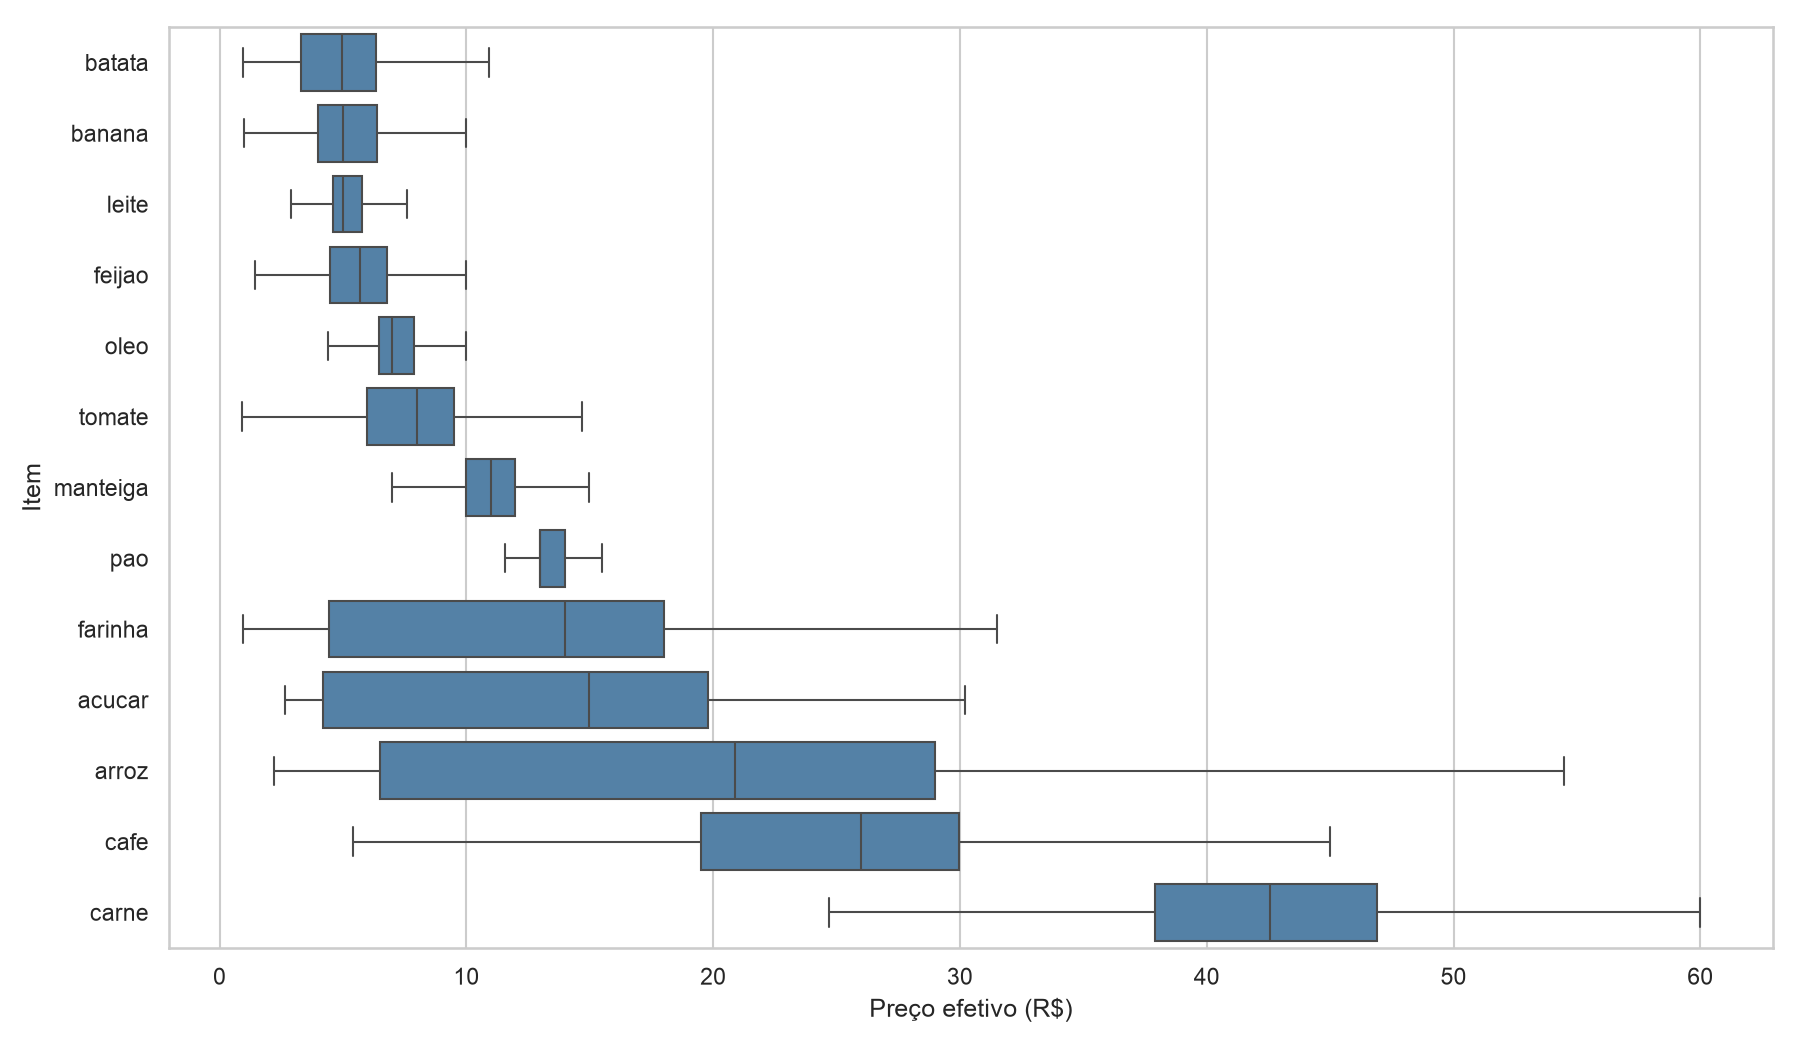
\includegraphics[width=\textwidth]{distribuicao_preco_por_item.png}
\end{figure}

A cobertura da pesquisa também é desigual entre redes: Condor, Jacomar e Atacadão lideram em número de registros na cesta (Figura~\ref{fig:redes}).

\begin{figure}[H]
\caption{Redes com mais registros na cesta básica (amostra)}
\label{fig:redes}
\centering
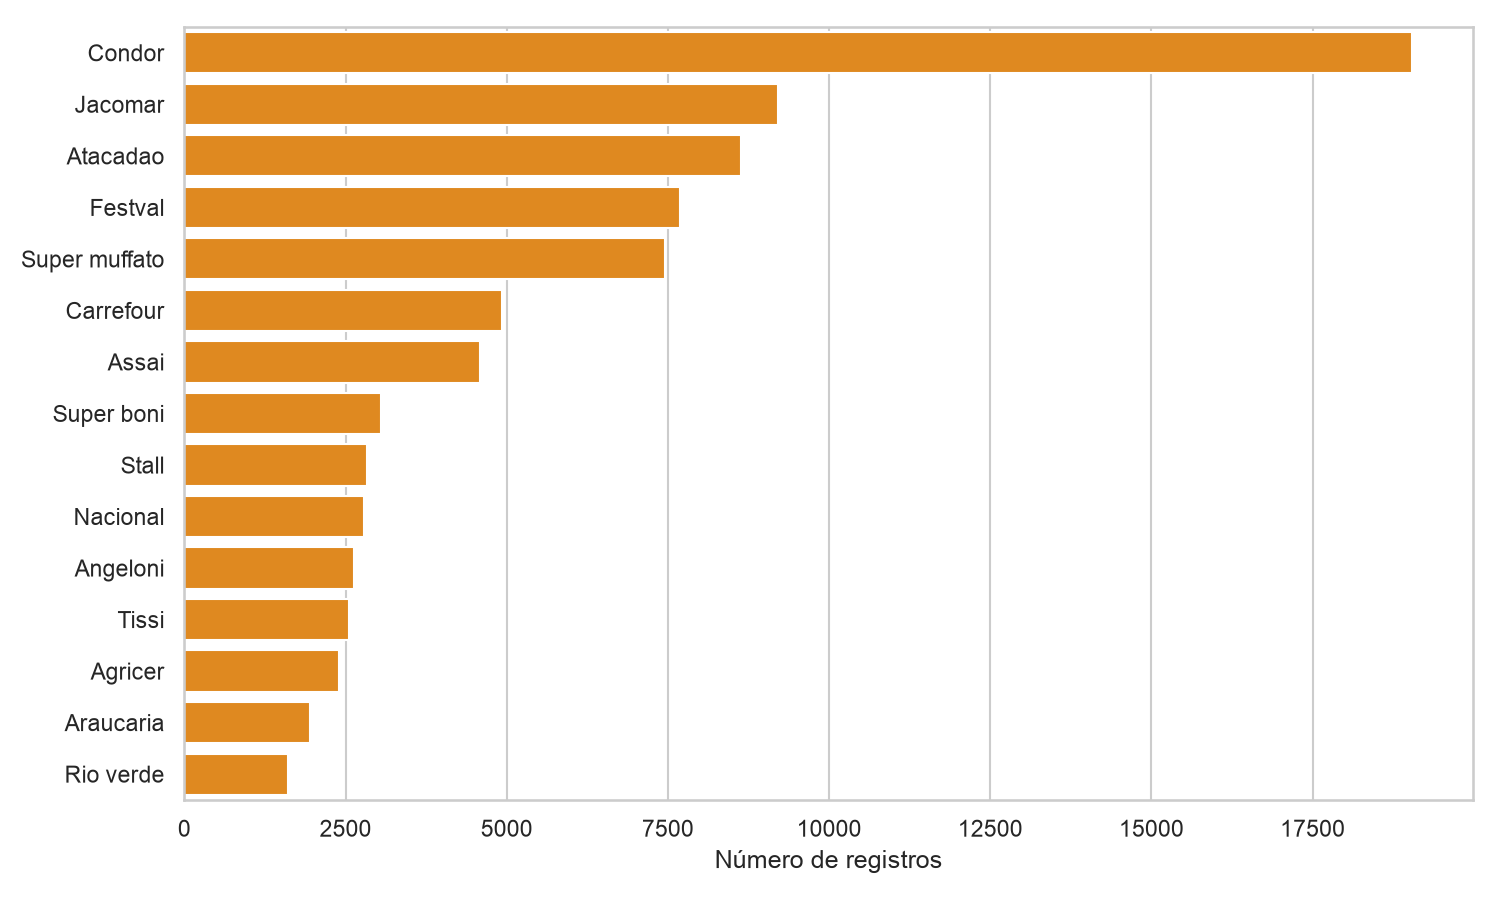
\includegraphics[width=0.8\textwidth]{top_redes.png}
\end{figure}

Só arroz, açúcar e farinha têm mais de um tamanho de embalagem na cesta (os demais 10 itens aparecem só em um tamanho). Nos três, o pacote de 5 kg sai mais barato por grama que o de 1 kg: a diferença é maior em farinha (cerca de 10\% mais barato no pacote grande) e menor em açúcar (cerca de 3\%). O arroz tem um comportamento misto: o pacote de 2 kg, bem mais raro na amostra, aparece com o menor preço por grama dos três tamanhos (Figura~\ref{fig:embalagem}).

\begin{figure}[H]
\caption{Preço por grama segundo o tamanho da embalagem (amostra)}
\label{fig:embalagem}
\centering
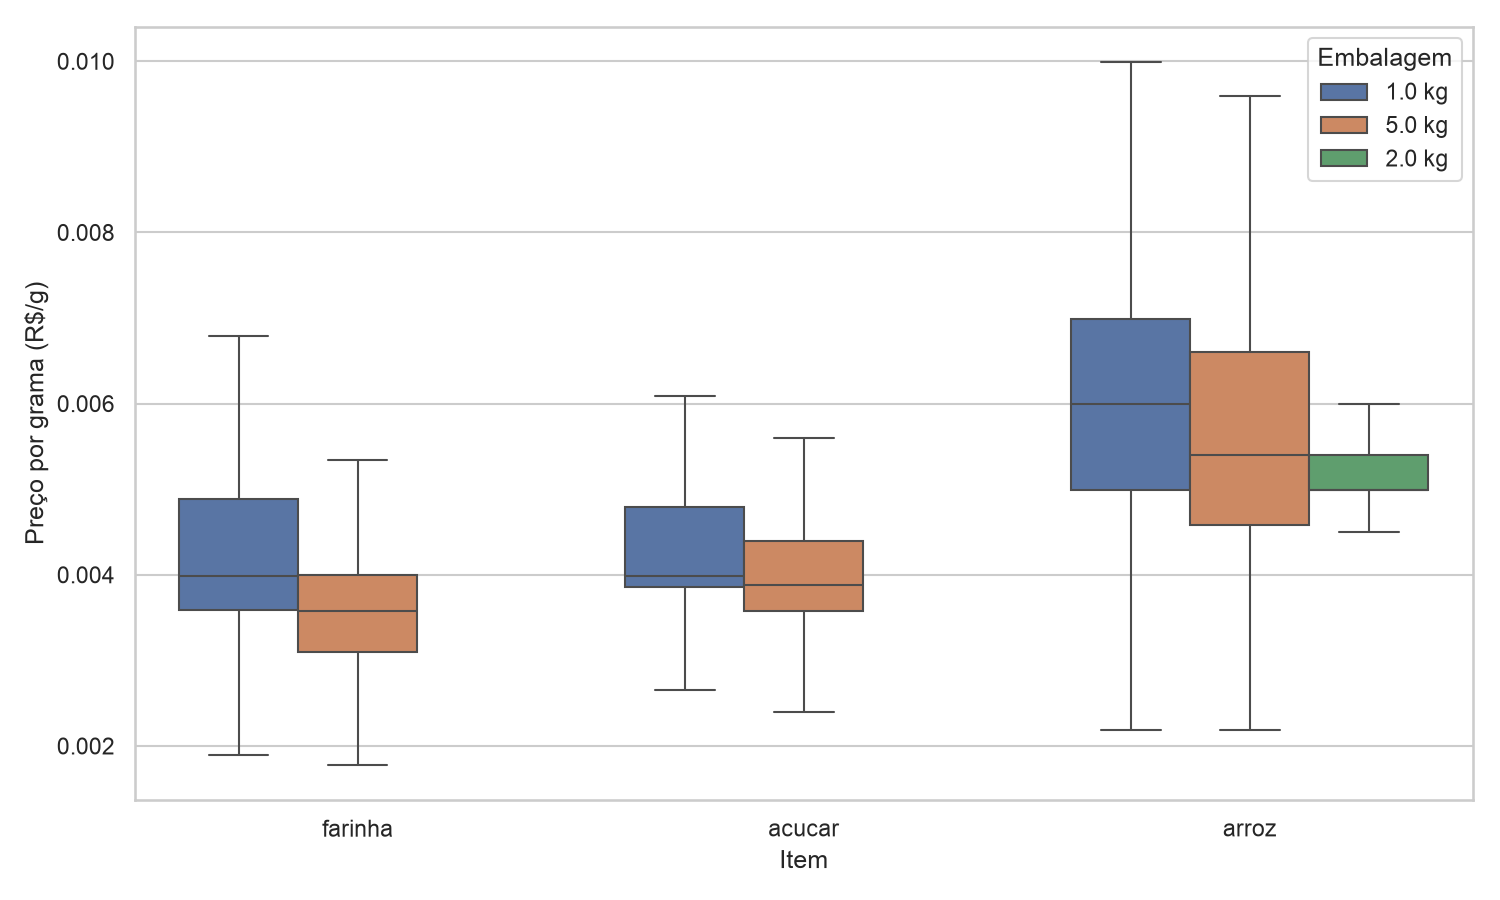
\includegraphics[width=\textwidth]{preco_por_unidade_embalagem.png}
\end{figure}

\section{Cesta básica: preparação, outliers e preço por unidade de medida}

\subsection{Seleção dos itens no conjunto completo}

A seção 6 do notebook, correspondente a esta seção do documento, repete sobre o conjunto completo, de forma independente da análise sobre a amostra, as mesmas decisões já tomadas e justificadas na seção 3:

\begin{itemize}[itemsep=2pt, topsep=2pt]
  \item \textbf{Identidade do produto por \col{id\_produto}, não por \col{descricao}}: a mesma descrição pode ter pequenas variações de grafia (seção 3.2), mas o código do produto é estável. Usar \col{id\_produto} evita que erros de digitação dividam o mesmo produto em grupos diferentes.
  \item \textbf{Rede normalizada pelo mesmo critério de similaridade e substring da seção 3.4}: sem um identificador único de rede, uma regra automática de agrupamento por nome poderia juntar redes diferentes ou separar a mesma rede; por isso a normalização é feita por comparação de pares de nomes, com as duas exceções já verificadas manualmente.
  \item \textbf{\col{preco\_efetivo} com a mesma prioridade da seção 3.3} (promoção, regular, fidelidade, atacado): a promoção tem prioridade por ser o preço que qualquer cliente paga durante a oferta; regular vem em seguida porque nem toda rede pratica atacado ou fidelidade, e não é correto assumir que todas as compras ocorram nessas condições.
  \item \textbf{Remoção dos registros sem nenhum preço preenchido}: na exploração da amostra (seção 3.3) esses registros foram mantidos, mas, como não é possível calcular custo sem preço, a análise da cesta básica os remove.
  \item \textbf{Seleção dos 13 itens e do subtipo exigido pela metodologia do DIEESE, decidida por \col{id\_produto}}: os produtos no dataset têm diversas variedades (por exemplo, carne com corte comum ou nobre), mas a metodologia da Cesta Básica de Alimentos especifica qual variedade de cada item compõe a cesta oficial (seção 3.6); decidir por \col{id\_produto}, e não por linha, evita que um erro de digitação exclua parte dos registros de um produto já incluído.
  \item \textbf{Correção dos três erros de digitação no fracionamento} (seção 4.2) e \textbf{corte a partir de abril de 2023} (seção 4.2): necessários para que o tamanho de embalagem exista e seja interpretado corretamente em todos os registros usados.
  \item \textbf{Remoção de outliers por IQR (k=1,5)}: mesmo critério e mesma justificativa da seção 3.5, aplicado por item para não misturar a faixa de preço de produtos diferentes.
\end{itemize}

Nenhuma regra nova entra nesta etapa: o objetivo é aplicar, ao conjunto completo, o que já foi validado na amostra. A seleção inicial dos 13 itens no conjunto completo resulta em 463 produtos e 1.267.450 registros; depois da exigência de preço válido e do corte de data (seção 4.2), restam 1.030.412 registros; depois da seleção do subtipo específico de cada item e da extração do tamanho de embalagem, restam 474.180 registros em 13 produtos-tipo; a remoção de outliers por IQR deixa 470.333 registros.

\subsection{Corte de data e extração do tamanho da embalagem}

Até março de 2023, a pesquisa registrava os itens de forma genérica, sem marca nem tamanho de embalagem (por exemplo, ``Arroz polido''). A partir de abril de 2023, os registros passaram a trazer essa informação no final da descrição, separada por um hífen. Sem o tamanho, \col{qtd\_fracionamento} fica vazio e o preço por quilo não pode ser calculado nem comparado dentro do mesmo grupo de embalagem; por isso a cesta básica usa somente registros a partir de abril de 2023.

A extração do tamanho exigiu corrigir três padrões de erro de preenchimento encontrados nos dados: ``1 gr''/``1 ml'' tratados como ``1 kg''/``1 litro'', porque nenhum item da cesta é vendido em pacote de 1 grama ou mililitro; ``5 gr'' em farinha tratado como ``5 kg'', porque a farinha não é vendida em pacote de 5 gramas; e ``- -kg'' sem número (hífen duplicado por falha de formatação, caso do pão francês vendido a granel), tratado como ``1 kg''.

\subsection{Preço por unidade de medida}

O \col{qtd\_fracionamento} (em g ou ml) é convertido para a unidade de medida que a metodologia do DIEESE usa em cada item: quilograma para a maioria, litro para leite e óleo. A metodologia (DIEESE, 2025a) trata a banana como um caso especial: para supermercados, sacolões e hortifrútis, onde o preço é coletado por quilo, a metodologia multiplica esse preço por 1,2 (prata) ou 1,8 (nanica/caturra); já nas feiras, o preço já é coletado por dúzia e não recebe esse multiplicador. Esses dois valores, 1,2 kg e 1,8 kg, correspondem ao peso aproximado de uma dúzia de cada variedade, de modo que o resultado da multiplicação é o preço por dúzia, não por banana individual. Com o preço mediano real de R\$ 4,99 a R\$ 5,99 por quilo (prata/caturra), o multiplicador resulta em algo entre R\$ 6 e R\$ 11 por dúzia, valor plausível para o item; interpretado como preço por banana individual, passaria de R\$ 10 por uma única fruta, o que não é.

Com o preço convertido para a unidade correta, a série mensal de cada item mostra evoluções bem diferentes entre si: o café, por exemplo, mais que dobrou de preço entre abril de 2023 e o pico em junho de 2025, enquanto a farinha teve variação muito menor no mesmo período (Figuras~\ref{fig:unidade-1} a \ref{fig:unidade-7}).

\begin{figure}[H]
\caption{Preço por unidade de medida ao longo do tempo (1/7)}
\label{fig:unidade-1}
\centering
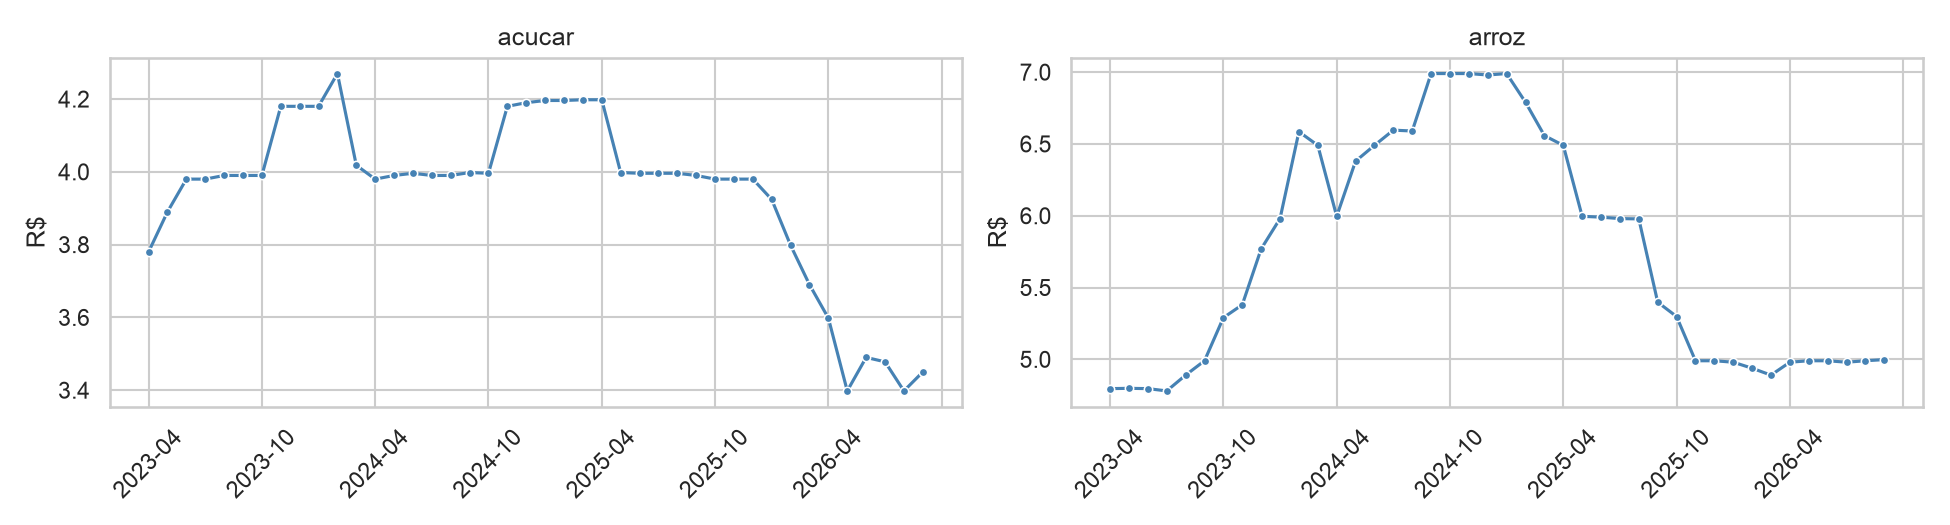
\includegraphics[width=\textwidth]{cesta_preco_por_unidade_acucar_arroz.png}
\end{figure}

\begin{figure}[H]
\caption{Preço por unidade de medida ao longo do tempo (2/7)}
\label{fig:unidade-2}
\centering
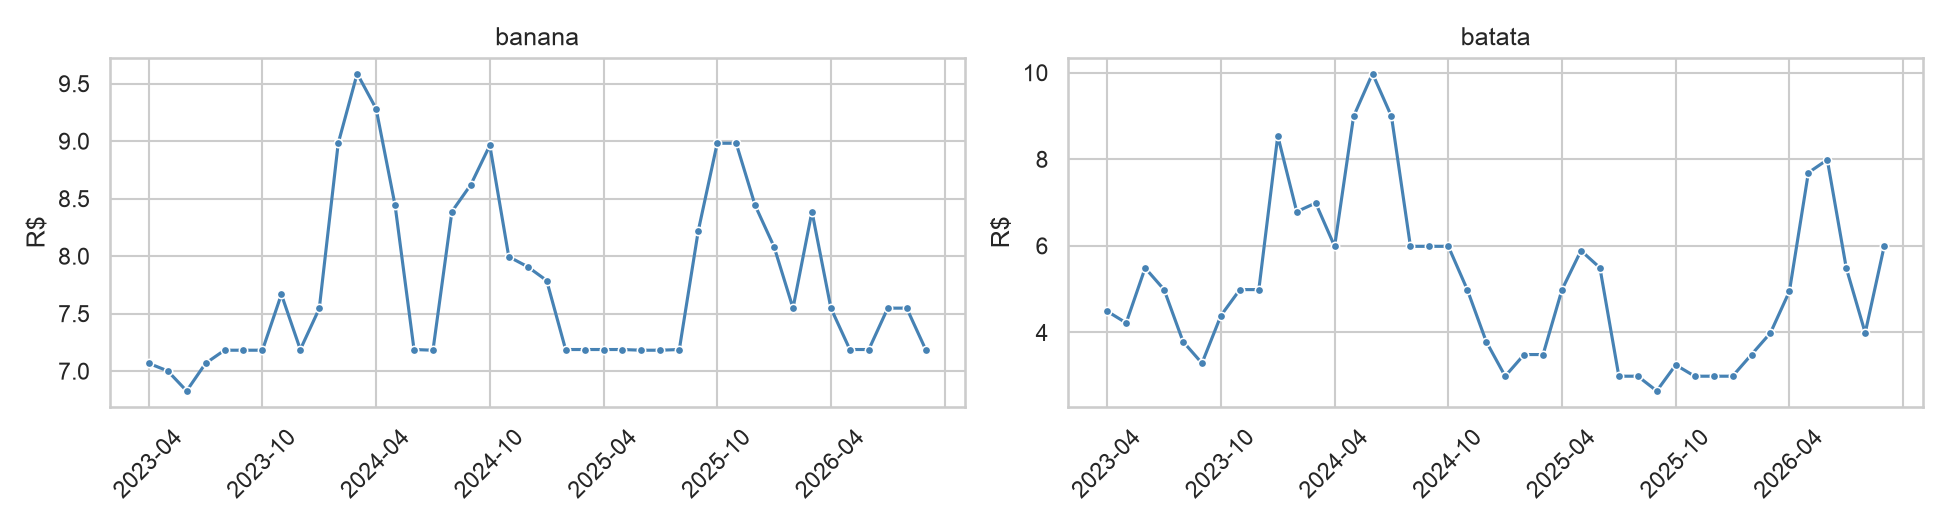
\includegraphics[width=\textwidth]{cesta_preco_por_unidade_banana_batata.png}
\end{figure}

\begin{figure}[H]
\caption{Preço por unidade de medida ao longo do tempo (3/7)}
\label{fig:unidade-3}
\centering
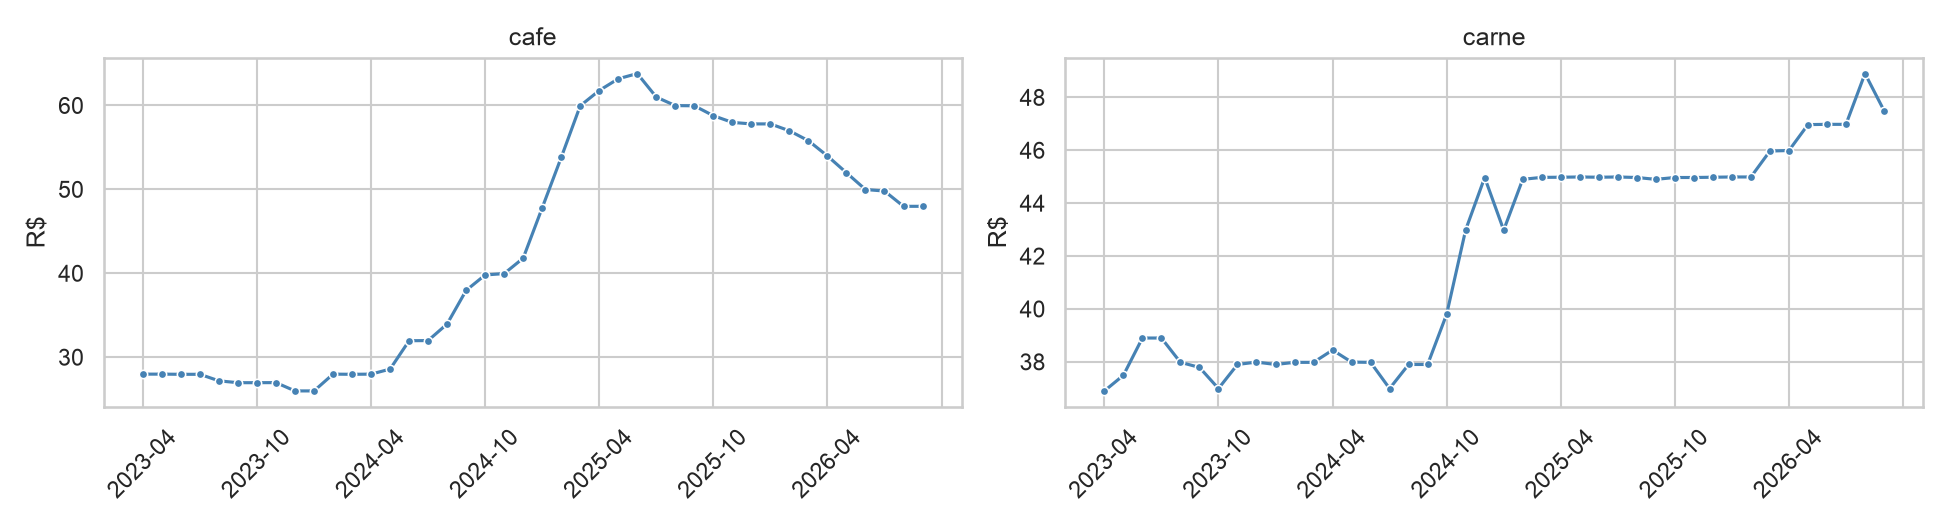
\includegraphics[width=\textwidth]{cesta_preco_por_unidade_cafe_carne.png}
\end{figure}

\begin{figure}[H]
\caption{Preço por unidade de medida ao longo do tempo (4/7)}
\label{fig:unidade-4}
\centering
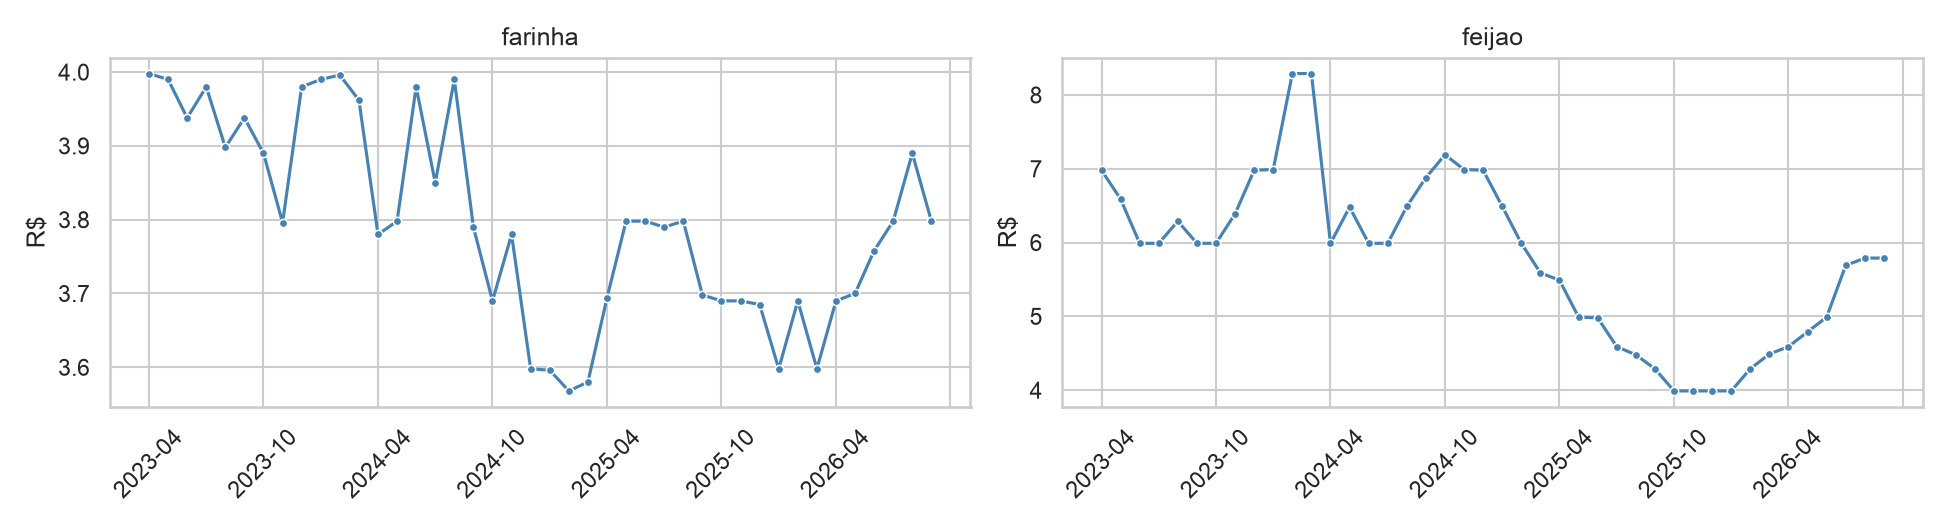
\includegraphics[width=\textwidth]{cesta_preco_por_unidade_farinha_feijao.png}
\end{figure}

\begin{figure}[H]
\caption{Preço por unidade de medida ao longo do tempo (5/7)}
\label{fig:unidade-5}
\centering
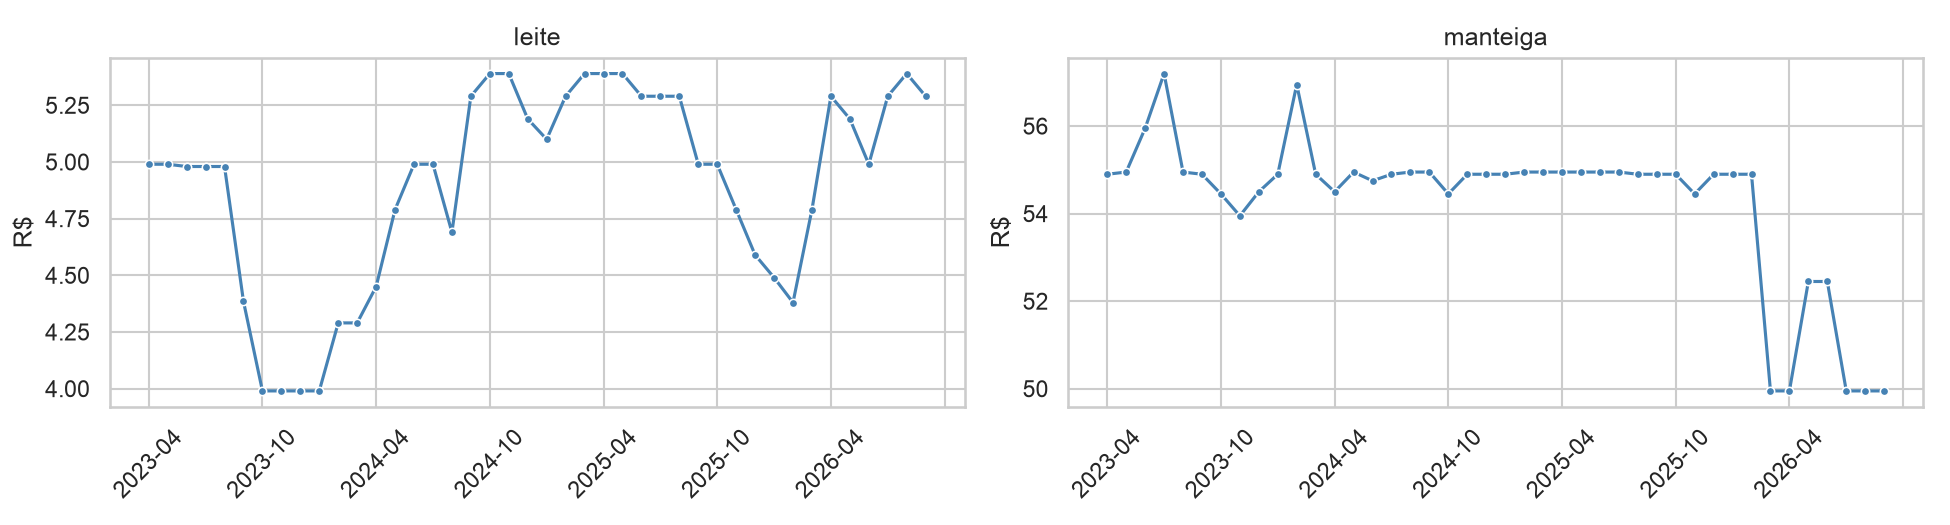
\includegraphics[width=\textwidth]{cesta_preco_por_unidade_leite_manteiga.png}
\end{figure}

\begin{figure}[H]
\caption{Preço por unidade de medida ao longo do tempo (6/7)}
\label{fig:unidade-6}
\centering
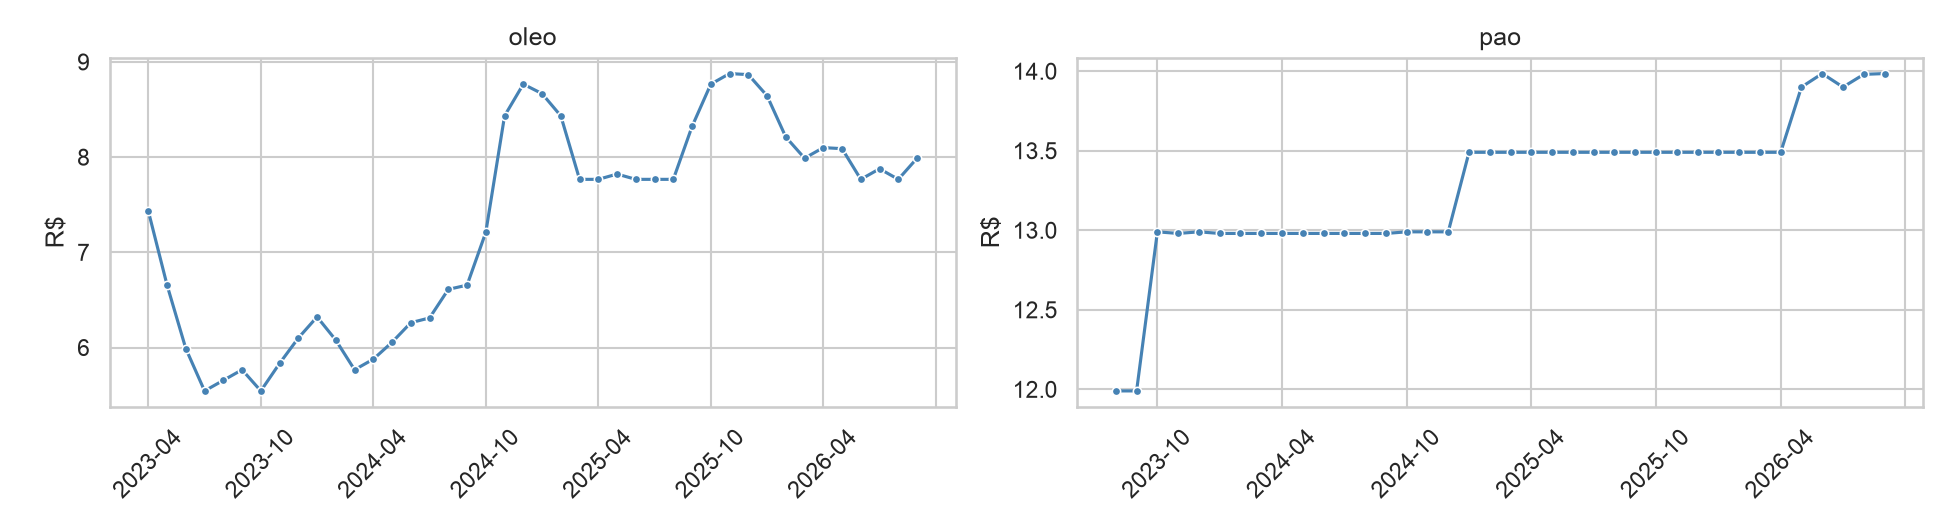
\includegraphics[width=\textwidth]{cesta_preco_por_unidade_oleo_pao.png}
\end{figure}

\begin{figure}[H]
\caption{Preço por unidade de medida ao longo do tempo (7/7)}
\label{fig:unidade-7}
\centering
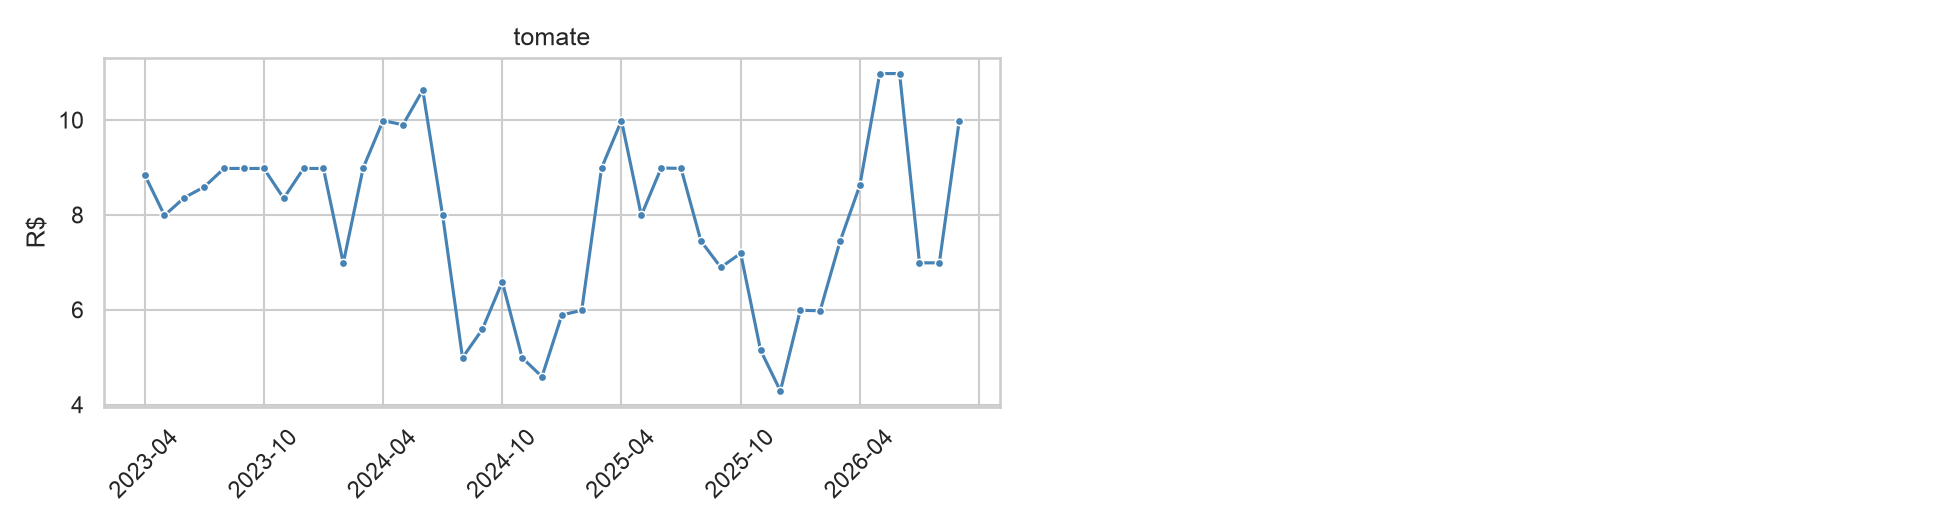
\includegraphics[width=\textwidth]{cesta_preco_por_unidade_tomate.png}
\end{figure}

\section{Custo da cesta básica}

\subsection{Quantidades por item}

O custo mensal da cesta multiplica o preço por unidade de medida de cada item pela quantidade mensal definida pelo Decreto-Lei n\textsuperscript{o} 399, de 1938, que a metodologia do DIEESE segue para todas as regiões do país (DIEESE, [20--]b; DIEESE, 2025a). As quantidades usadas são as da Região 3, que inclui o Paraná (Tabela~\ref{tab:quantidades}).

\begin{table}[H]
\caption{Quantidades mensais da cesta básica, Região 3 (Decreto-Lei n\textsuperscript{o} 399/1938)}
\label{tab:quantidades}
\small
\centering
\begin{tabular}{@{}lr@{}}
\toprule
\textbf{Item} & \textbf{Quantidade mensal} \\
\midrule
Carne & 6,6 kg \\
Leite & 7,5 l \\
Feijão & 4,5 kg \\
Arroz & 3,0 kg \\
Farinha & 1,5 kg \\
Batata & 6,0 kg \\
Tomate & 9,0 kg \\
Pão & 6,0 kg \\
Café & 0,6 kg \\
Banana & 7,5 dúzias (90 unidades) \\
Açúcar & 3,0 kg \\
Óleo & 0,9 l \\
Manteiga & 0,75 kg \\
\bottomrule
\end{tabular}
\end{table}

\subsection{Custo mensal}

O pão francês não tem nenhum registro com tamanho de embalagem reconhecido entre abril e julho de 2023, por isso o custo mensal da cesta nesses quatro meses é calculado com no mínimo 12 dos 13 itens disponíveis, o que subestima levemente o valor real nesse período. A partir de agosto de 2023, todos os 13 itens estão disponíveis todos os meses.

O custo da cesta sai de R\$ 568,35 em abril de 2023, sobe até um pico de R\$ 761,92 em junho de 2026 e fecha a série em R\$ 747,29 em setembro de 2026 (Figura~\ref{fig:custo-mensal}).

\begin{figure}[H]
\caption{Custo mensal da cesta básica em Curitiba}
\label{fig:custo-mensal}
\centering
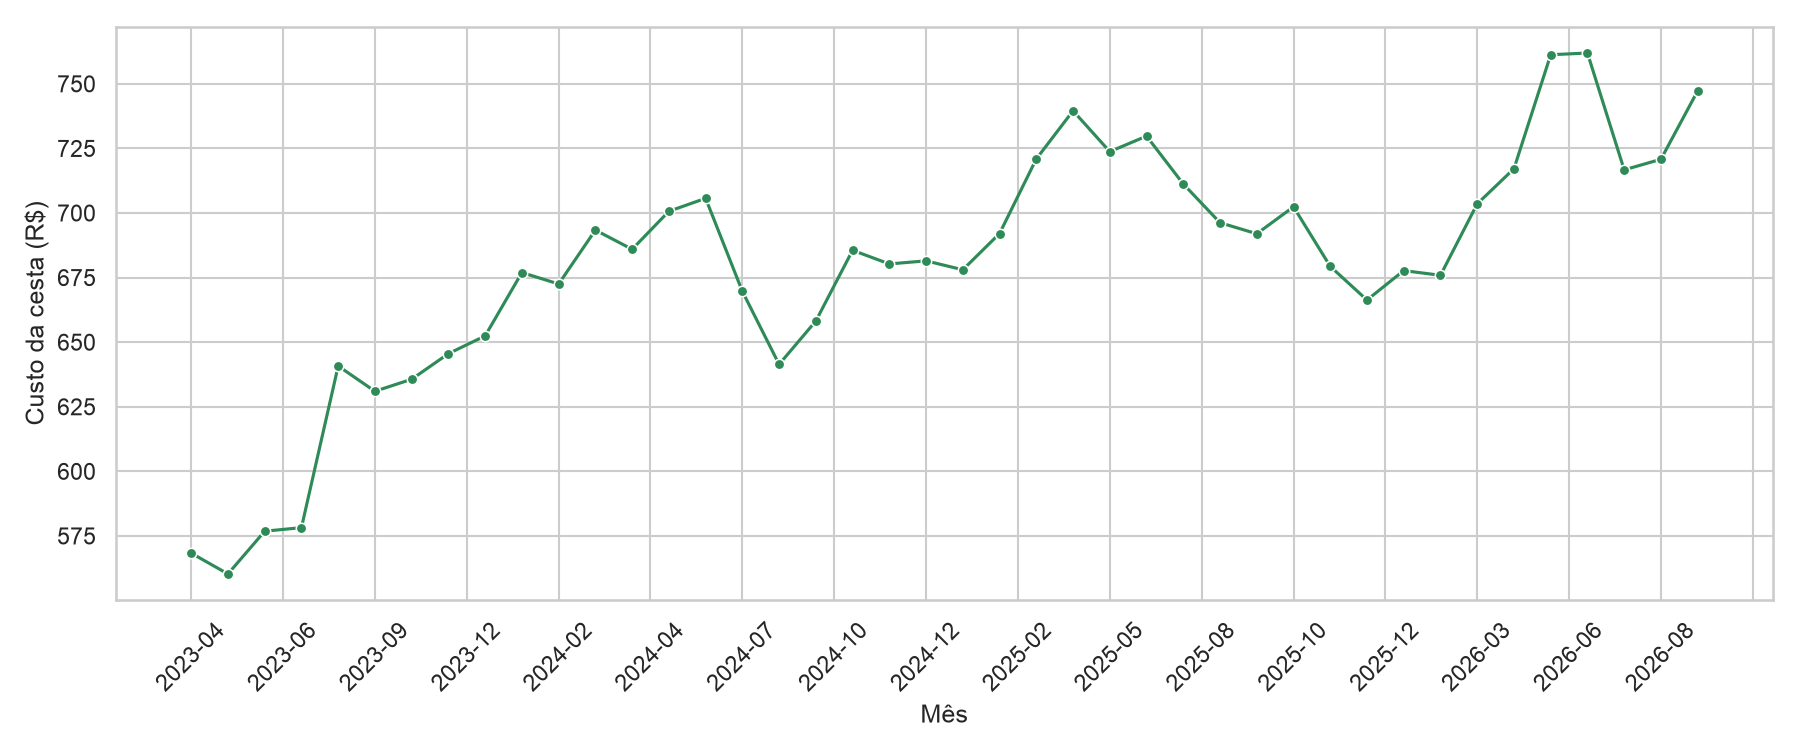
\includegraphics[width=\textwidth]{cesta_custo_mensal.png}
\end{figure}

\subsection{Contribuição de cada item para a variação do custo}

Como o custo da cesta é a soma de \col{preco\_unitario} multiplicado pela quantidade de cada item, a contribuição de cada item para a variação do custo em um período é exatamente essa multiplicação, aplicada à diferença de preço entre o início e o fim do período. Essa decomposição foi escolhida em vez de uma correlação entre os preços e o custo total, porque os itens são literalmente parcelas da soma que forma o custo, o que distorceria qualquer coeficiente de correlação calculado diretamente.

Entre agosto de 2023 (primeiro mês com os 13 itens disponíveis) e setembro de 2026, carne foi, isoladamente, o item que mais empurrou o custo da cesta para cima, seguido por tomate, café e pão, com contribuições parecidas entre si. Manteiga foi o item com maior contribuição negativa no período, seguida de açúcar e feijão, com contribuições negativas bem menores (Figura~\ref{fig:contribuicao}).

\begin{figure}[H]
\caption{Contribuição de cada item para a variação do custo da cesta (agosto/2023 a setembro/2026)}
\label{fig:contribuicao}
\centering
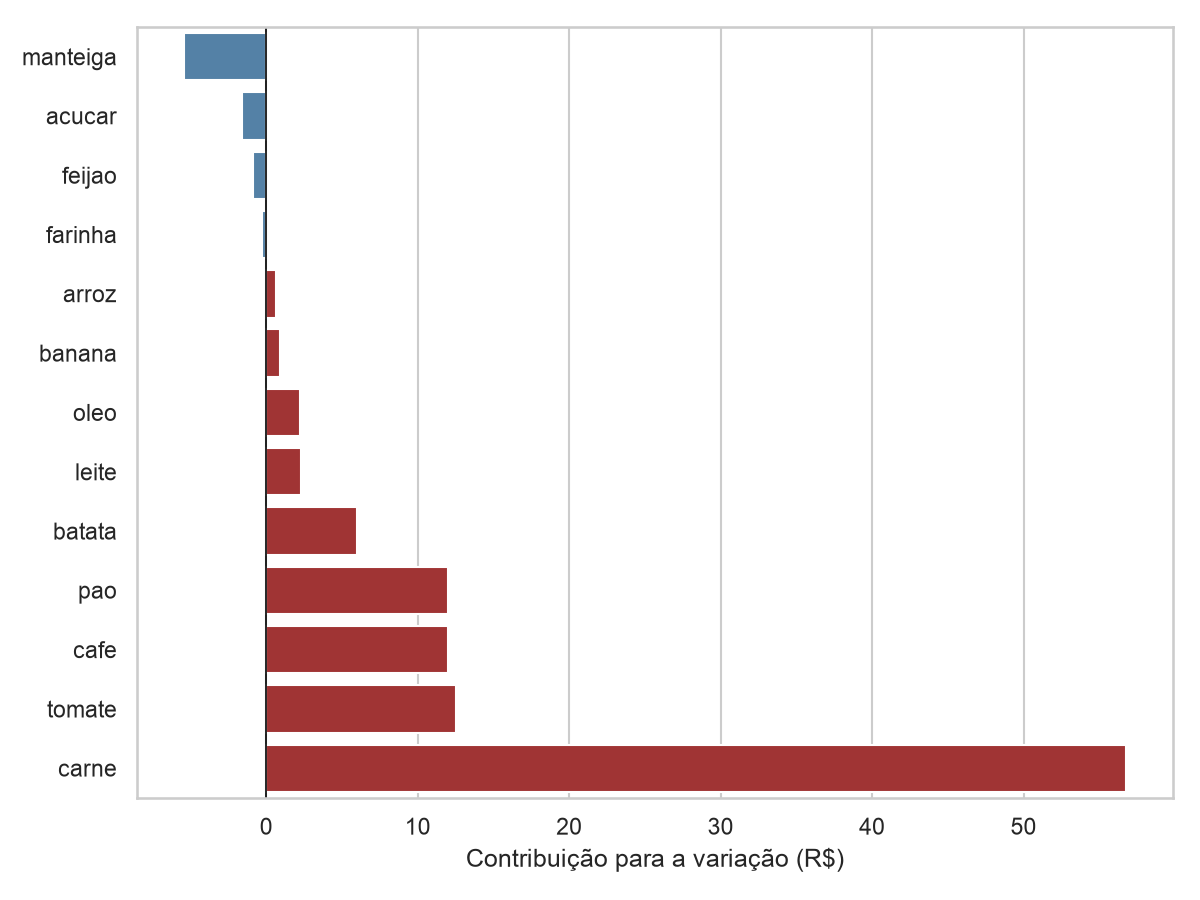
\includegraphics[width=0.75\textwidth]{cesta_contribuicao_periodo_completo.png}
\end{figure}

\subsection{Custo da cesta por rede}

A comparação do custo da cesta entre redes, nos últimos 12 meses da série, exige que a rede tenha pelo menos 20 registros de cada um dos 13 itens, para que a mediana de preço de cada item não fique instável com poucos pontos. Esse critério deixa de fora as redes de menor volume na pesquisa, que não necessariamente têm o mesmo perfil de preço das redes maiores: das 47 redes normalizadas ativas no período, 20 (42,6\%) atendem ao critério.

Entre essas 20 redes, a cesta custou de R\$ 666,68 na Super Boni a R\$ 776,47 na Rede Master, uma diferença de 16,5\% (Figura~\ref{fig:custo-rede}).

\begin{figure}[H]
\caption{Custo da cesta por rede, últimos 12 meses da série (redes elegíveis)}
\label{fig:custo-rede}
\centering
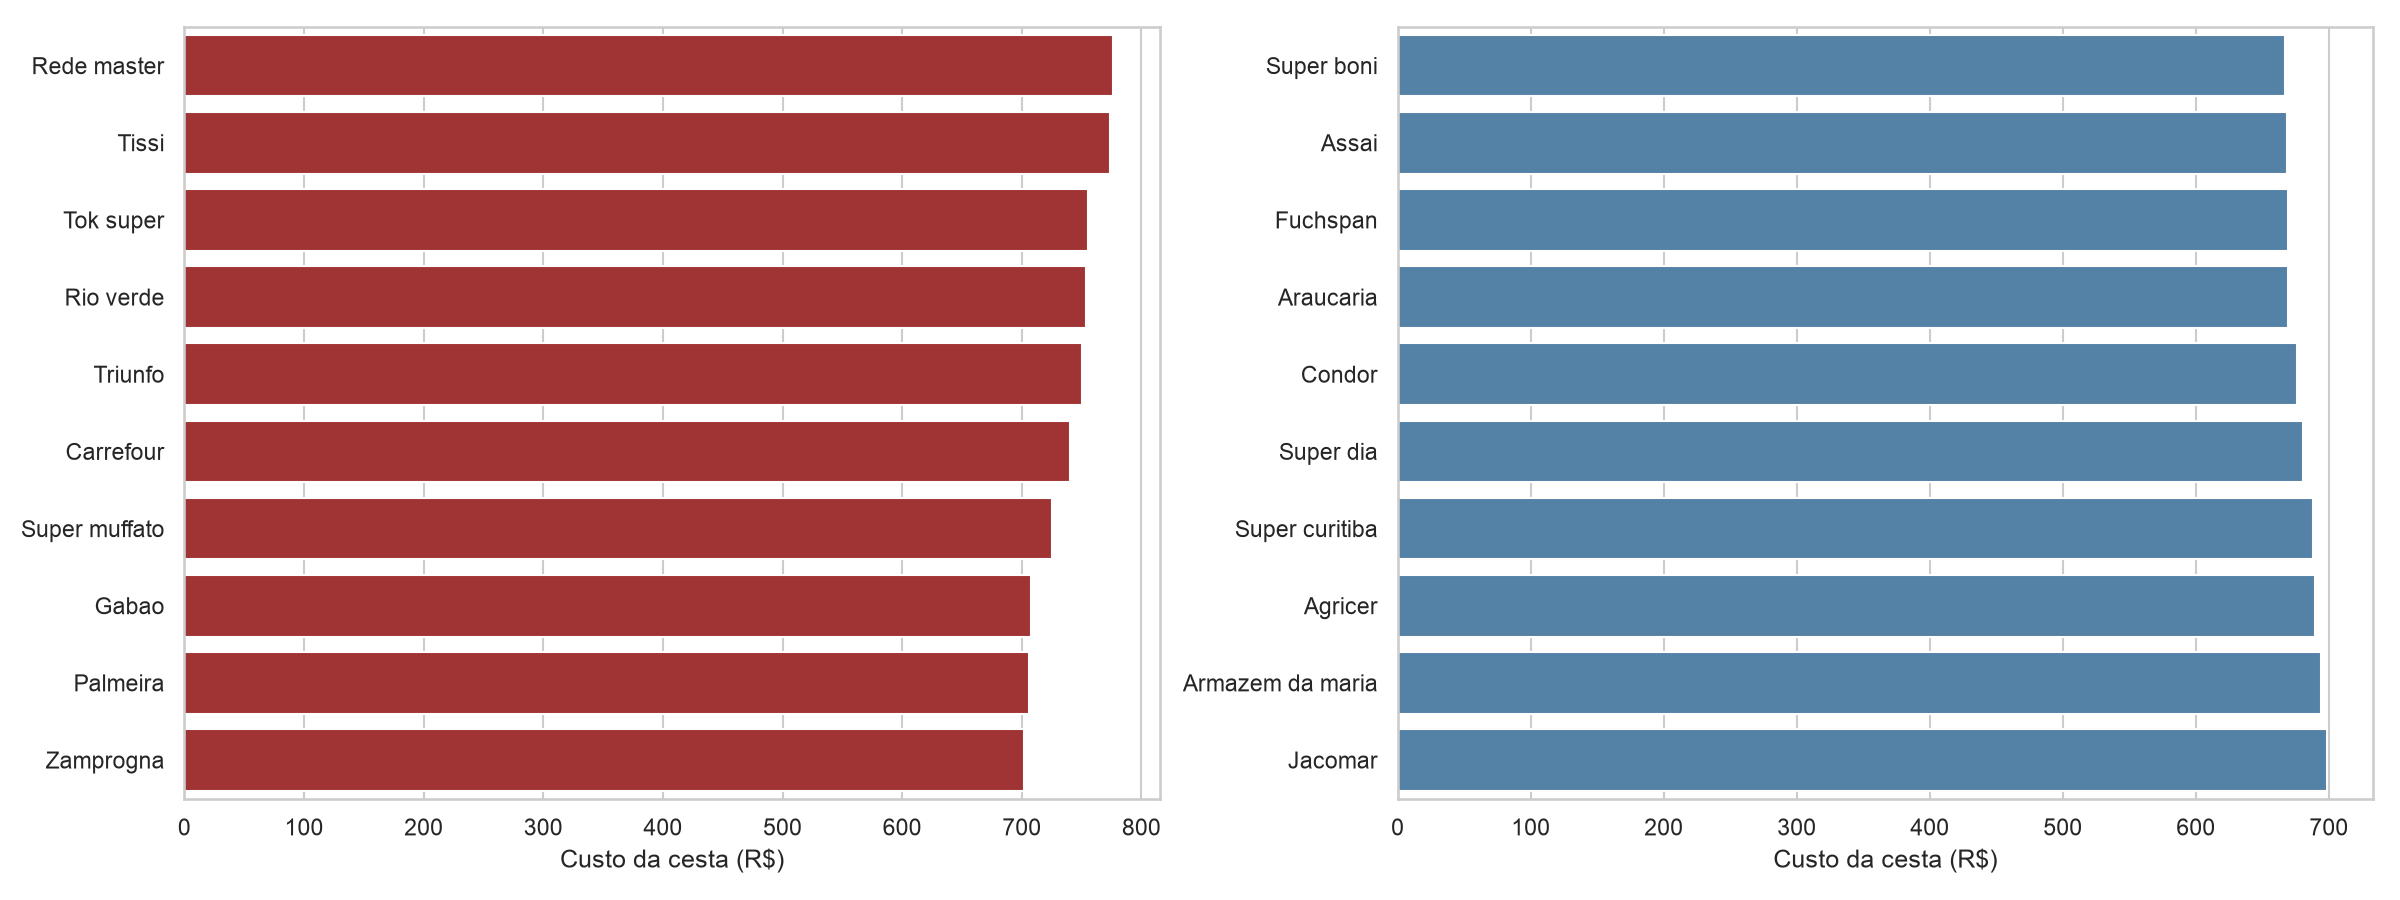
\includegraphics[width=\textwidth]{cesta_custo_por_rede.png}
\end{figure}

Como a mediana de cada item reúne todos os tipos e marcas vendidos na rede, parte da diferença entre redes pode vir do mix de produtos que cada uma vende, e não só do preço cobrado pelo mesmo produto.

\subsection{Evolução do custo nas redes com mais registros}

Diferente da comparação da seção 5.4, que usa só os últimos 12 meses e exige volume mínimo por item, esta seção acompanha a série histórica completa, restrita às cinco redes com mais registros na cesta básica. O filtro de volume mínimo não é necessário aqui, porque essas redes já têm volume alto por construção (Figura~\ref{fig:custo-top5}).

\begin{figure}[H]
\caption{Evolução do custo da cesta nas cinco redes com mais registros}
\label{fig:custo-top5}
\centering
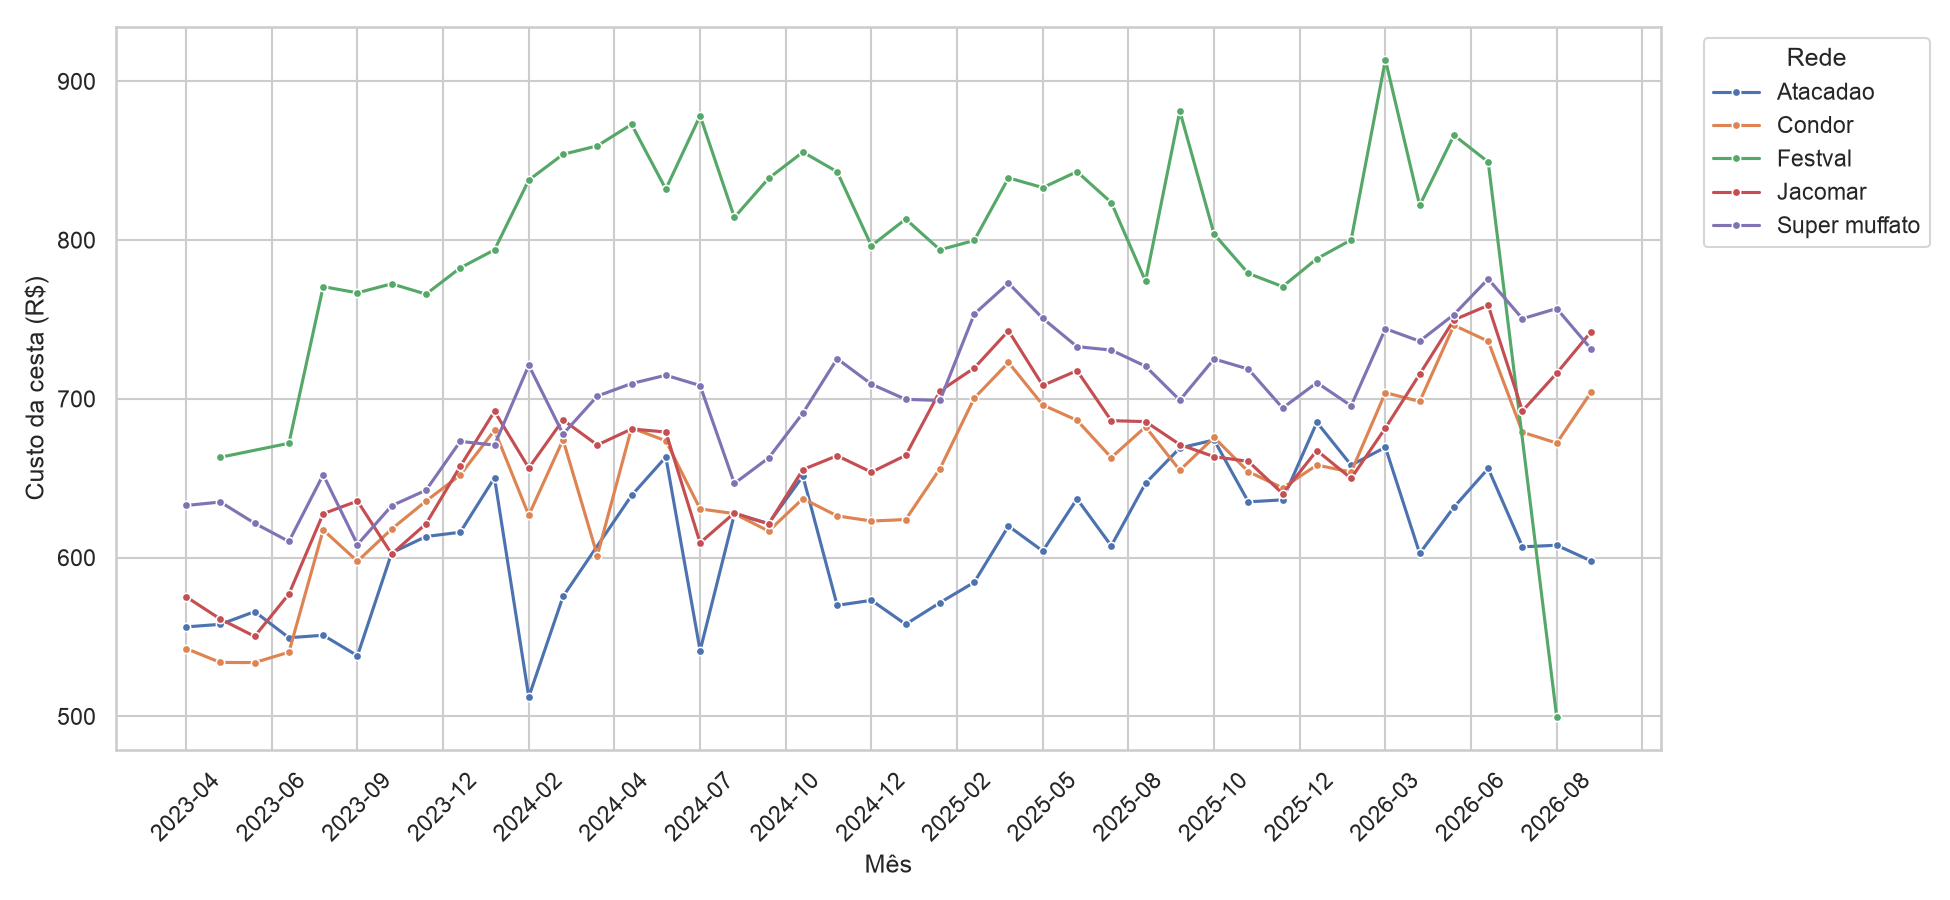
\includegraphics[width=\textwidth]{cesta_custo_top5_redes.png}
\end{figure}

\section{Considerações finais}

A base é grande e quase completa: só duas colunas têm ausentes, e nenhuma é central para o estudo. Os cuidados estão em outros pontos: preços sobrepostos, resolvidos com o preço efetivo; identificador de filial que não é único; nomes de rede inconsistentes; alguns preços impossíveis, já removidos; a troca de formato de descrição em março de 2023, que deixa a comparação por unidade de medida possível só a partir de abril daquele ano; e a cobertura desigual entre redes, que limita a comparação de custo por rede a uma fração delas.

Com os 13 itens da cesta básica padronizados pela metodologia do DIEESE, o custo da cesta em Curitiba teve pico de R\$ 761,92 em junho de 2026 e fechou setembro de 2026 em R\$ 747,29. Nos últimos 12 meses, entre as redes com volume suficiente para comparação, a mesma cesta custou de R\$ 666,68 a R\$ 776,47, uma diferença de 16,5\% que o consumidor não vê na consulta diária do Clique Economia. Carne foi, isoladamente, o item que mais pressionou essa alta no período completo da série, seguida por tomate, café e pão; manteiga foi o item que mais ajudou a conter o custo.

% =====================================================================
% POS-TEXTUAIS
% =====================================================================
\section*{Referências}

\begin{singlespace}
\setlength{\parindent}{0pt}
\setlength{\parskip}{12pt}

BRASIL. Decreto-Lei n\textsuperscript{o} 399, de 30 de abril de 1938. Regula o disposto no Capítulo I, Título III, da Consolidação das Leis do Trabalho, no tocante a salário mínimo, e dá outras providências. \textit{Diário Oficial da União}, Rio de Janeiro, 30 abr. 1938.

DIEESE. \textit{Metodologia da cesta básica nacional}. São Paulo, [20--]b. Disponível em: \url{https://www.dieese.org.br/metodologia/metodologiaCestaBasica.html}. Acesso em: 2 out. 2026.

DIEESE. \textit{Metodologia da Pesquisa Nacional da Cesta Básica de Alimentos}. São Paulo, 2025a. Disponível em: \url{https://www.dieese.org.br/metodologia/metodologiaCestaBasica2025.html}. Acesso em: 2 out. 2026.

DIEESE. \textit{Em maio, custo da cesta aumenta em todas as 27 capitais analisadas}. São Paulo, 2026. Disponível em: \url{https://www.dieese.org.br/analisecestabasica/2026/202605cestabasica.html}. Acesso em: 2 out. 2026.

PAULOGLADSON. \textit{Clique Economia Dados (Curitiba)}. [\textit{S.~l.}]: Kaggle, [20--]. Disponível em: \url{https://www.kaggle.com/datasets/paulogladson/clickeconomiadados}. Acesso em: 1 out. 2026.

PREFEITURA de Curitiba. \textit{Clique Economia}. Curitiba, [20--]. Disponível em: \url{https://www.curitiba.pr.gov.br/noticias/do-clique-economia-aos-armazens-da-familia-conheca-os-aliados-do-consumidor-de-curitiba/67679}. Acesso em: 1 out. 2026.
\end{singlespace}

\section*{Glossário}

\begin{description}[style=standard, leftmargin=0pt, itemsep=3pt, font=\normalfont\bfseries]
\item[AED:] Análise exploratória de dados.
\item[Amostra:] Subconjunto de registros sorteado do conjunto completo. Aqui, cerca de 10\% dos registros, sorteados com semente fixa para que o resultado se repita.
\item[Assimetria à direita:] Distribuição em que poucos valores muito altos puxam a média para cima, deixando-a acima da mediana.
\item[Bloco (\textit{chunk}):] Parte do arquivo lida de cada vez, usada para processar o conjunto inteiro sem carregá-lo todo na memória.
\item[Cesta básica:] Conjunto padrão de alimentos usado como referência para medir o custo da alimentação de uma família.
\item[Coeficiente de variação:] Razão entre o desvio padrão e a média. Mede a dispersão relativa e permite comparar variáveis de escalas diferentes.
\item[Dados abertos:] Dados públicos disponibilizados para livre consulta e reutilização.
\item[Decreto-Lei n\textsuperscript{o} 399/1938:] Norma federal que define a composição e as quantidades mensais da cesta básica de alimentos por região do país, usada como referência pela metodologia do DIEESE.
\item[DIEESE:] Departamento Intersindical de Estatística e Estudos Socioeconômicos, responsável pela Pesquisa Nacional da Cesta Básica de Alimentos.
\item[EAN-13:] Padrão de código de barras de 13 dígitos usado para identificar produtos no varejo.
\item[Intervalo interquartil:] Diferença entre o terceiro e o primeiro quartil. Concentra a metade central dos dados e é a base do critério de outliers usado neste trabalho.
\item[IQR:] Intervalo interquartil (\textit{interquartile range}).
\item[LGPD:] Lei Geral de Proteção de Dados Pessoais.
\item[Notebook Jupyter:] Arquivo que combina código, resultados e texto explicativo, executado célula a célula.
\item[ODS:] Objetivos de Desenvolvimento Sustentável, da ONU.
\item[Outlier:] Valor muito distante dos demais. Pode ser erro de coleta ou um valor legítimo e raro.
\item[\textit{Pipeline} de dados:] Sequência de etapas pela qual os dados passam, da leitura até o resultado final.
\item[Preço efetivo:] Coluna criada pelo grupo com um único preço por registro, escolhido entre promoção, regular, fidelidade e atacado, nessa ordem.
\item[Preço por unidade de medida:] Preço efetivo dividido pelo tamanho da embalagem, convertido para quilograma, litro ou dúzia, conforme o item.
\item[Quartil:] Separatriz que divide os dados ordenados em 4 partes iguais. $Q_1$ marca os 25\% menores valores e $Q_3$ os 75\% menores.
\item[Rede:] Empresa de supermercados que pode ter várias lojas (filiais).
\item[Rede normalizada:] Nome da rede corrigido para eliminar variações de grafia e duplicidade do mesmo nome.
\item[Série temporal:] Sequência de valores medidos em intervalos regulares de tempo, como a mediana mensal de um preço.
\item[SMSAN:] Secretaria Municipal de Segurança Alimentar e Nutricional de Curitiba.
\end{description}

\end{document}
